\documentclass[journal]{IEEEtran}

% === Packages ===
\usepackage[utf8]{inputenc}
\usepackage[T1]{fontenc}
\usepackage{amsmath,amssymb}
\usepackage{graphicx}
\usepackage{booktabs}
\usepackage{multirow}
\usepackage{array}
\usepackage{cite}
\usepackage{url}
\usepackage{hyperref}
\hypersetup{
  colorlinks=true,
  linkcolor=black,
  citecolor=black,
  urlcolor=blue!70!black,
  pdftitle={CropPlanner: An AI-Powered Web Application for Crop Planning Recommendations},
  pdfauthor={Thatt Bunnag, Nathanon Ratchathornbuathip, Art-ong Mukngoen, Atthaphon Lorphan},
}
\usepackage{xcolor}
\usepackage{microtype}
\usepackage{balance}
\usepackage[caption=false]{subfig}
\usepackage{tikz}
\usetikzlibrary{shapes.geometric, arrows.meta, positioning, fit, calc, backgrounds, decorations.pathreplacing, patterns}
\usepackage{pgfplots}
\usepgfplotslibrary{groupplots,dateplot}
\pgfplotsset{compat=1.18}
\usepackage[ruled,vlined,linesnumbered]{algorithm2e}
\usepackage{tabularx}
\graphicspath{{./}{../fig/}}

% === TikZ styles ===
\tikzset{
  % Flowchart styles
  startstop/.style={rectangle, rounded corners=6pt, minimum width=2.4cm, minimum height=0.7cm, text centered, draw=black, fill=green!15, font=\scriptsize},
  process/.style={rectangle, minimum width=2.8cm, minimum height=0.7cm, text centered, draw=black, fill=blue!8, font=\scriptsize},
  decision/.style={diamond, aspect=2.2, minimum width=1.2cm, minimum height=0.6cm, text centered, draw=black, fill=orange!15, font=\scriptsize},
  io/.style={trapezium, trapezium left angle=70, trapezium right angle=110, minimum width=2cm, minimum height=0.6cm, text centered, draw=black, fill=yellow!12, font=\scriptsize},
  arrow/.style={-{Stealth[length=2mm]}, thick},
  % Architecture diagram styles
  block/.style={rectangle, rounded corners=3pt, minimum width=1.6cm, minimum height=0.6cm, text centered, draw=black, fill=#1, font=\scriptsize},
  block/.default={blue!12},
  smallblock/.style={rectangle, rounded corners=2pt, minimum width=1.2cm, minimum height=0.5cm, text centered, draw=black, fill=#1, font=\tiny},
  smallblock/.default={blue!12},
  bigblock/.style={rectangle, rounded corners=4pt, minimum width=2.2cm, minimum height=0.7cm, text centered, draw=black, fill=#1, font=\scriptsize},
  bigblock/.default={blue!12},
  group/.style={rectangle, rounded corners=4pt, draw=gray, dashed, inner sep=6pt},
}



\begin{document}

% === Title ===
\title{CropPlanner: An AI-Powered Web Application for Crop Planning Recommendations}

\author{
  \IEEEauthorblockN{Thatt Bunnag\IEEEauthorrefmark{1}, Nathanon Ratchathornbuathip\IEEEauthorrefmark{1}, Art-ong Mukngoen\IEEEauthorrefmark{2}, Atthaphon Lorphan\IEEEauthorrefmark{2}} \\
  \IEEEauthorblockA{Chitralada School, Bangkok, Thailand \\
  \IEEEauthorrefmark{1}Students \quad \IEEEauthorrefmark{2}Advisors}
}

\maketitle

% ============================================================
% ABSTRACT
% ============================================================
\begin{abstract}
Agricultural price volatility exceeding 20\% annually, combined with the prevalence of monoculture farming practices, exposes Thai farmers to significant income risks. This paper presents CropPlanner, an integrated system comprising three components: (1)~a comparative study of AI models for 12-month crop price forecasting, including LSTM, Transformer, ARIMA, and a proposed Rolling-Window LSTM; (2)~a crop planning recommendation system formulated as a Weighted Job Scheduling Problem solved by a Greedy Heuristic; and (3)~a web application for farmers. Experiments were conducted using 20~years of monthly price data (2004--2024) for four major field crops---cassava, corn, green bean, and soybean---in Northeastern Thailand. Results show that no single model dominates across all crops: Standard LSTM achieved the highest average accuracy of 92.93\%, while Rolling-Window LSTM---with window sizes selected via a held-out validation year to prevent data leakage---achieved correct peak timing for two of four crops and within one month for a third, a property critical for scheduling. Exhaustive enumeration over all $4! = 24$ permutations identified the optimal non-overlapping four-crop rotation plan yielding 39,212~THB/rai/year, approximately 1.9~times the income of the best monoculture option, while revealing that the greedy heuristic is suboptimal by 14.8\%.
\end{abstract}

\begin{IEEEkeywords}
Machine Learning, Price Forecasting, Web Application, Time Series, ARIMA, LSTM, Transformer, Crop Planning
\end{IEEEkeywords}

% ============================================================
% I. INTRODUCTION
% ============================================================
\section{Introduction}

Agriculture forms a critical foundation of the Thai economy, contributing approximately 8\% of GDP while employing nearly 30\% of the workforce. Four major field crops---cassava, corn, green bean, and soybean---account for over 60\% of cultivated land and generate export revenues exceeding US\$13~billion annually~\cite{oae2024stats, oae2024forecast, ocsb2024, thairice2024}. However, prices of these crops exhibit significant volatility: cassava prices have fluctuated by up to 99\% year-over-year, corn experiences five or more high-volatility years per two decades, and green bean saw a 60\% single-year price surge in 2010~\cite{waqas2024climate}. This volatility, which exceeds 20\% within a 12-month period for most crops, creates substantial income risks for the approximately 5.7~million Thai agricultural households.

A key contributing factor is the widespread practice of monoculture farming. Many farmers plant the same crop continuously throughout the year, leaving them vulnerable when prices decline during certain periods~\cite{asg2014}. While government price support programs provide temporary relief, they are insufficient for long-term income stabilization. What farmers fundamentally lack are tools for forward-looking price forecasting and systematic planting schedule optimization.

Recent advances in machine learning, particularly time-series models such as LSTM~\cite{hochreiter1997lstm} and Transformer~\cite{vaswani2017attention}, have demonstrated significant improvements over traditional statistical methods for agricultural commodity price prediction~\cite{rohan2025crop}. Yet three critical gaps remain in the literature: (1)~most existing work forecasts individual crop prices in isolation, without connecting predictions to actionable planting recommendations~\cite{javaid2023ai}; (2)~\textit{peak timing accuracy}---the ability to predict \textit{when} prices peak---has not been evaluated as a distinct metric, despite being the most relevant property for scheduling harvest dates; and (3)~no prior system delivers an end-to-end pipeline from multi-model forecasting comparison through scheduling optimization to a farmer-accessible web interface.

This paper presents CropPlanner, an end-to-end system linking AI-based price forecasting with crop scheduling and a farmer-facing web application. Our contributions are threefold:

\begin{enumerate}
  \item \textbf{Model comparison and improvement:} We compare LSTM, Transformer, ARIMA, and a proposed Rolling-Window LSTM for 12-month price forecasting of four Thai field crops, analyzing both overall accuracy and peak timing accuracy. We demonstrate that the RW-LSTM addresses key limitations of standard models---off-peak prediction, long-range averaging, and structural break sensitivity---through a validated windowing approach.
  \item \textbf{Crop planning recommendation:} We formulate planting schedule optimization as a Weighted Job Scheduling Problem~\cite{clrs2009} and solve it with a Greedy Heuristic, verified by exhaustive enumeration over all $4! = 24$ permutations to quantify suboptimality.
  \item \textbf{Web application:} We develop CropPlanner, a prototype web application that presents forecasting results and planting recommendations through intuitive visualizations accessible to non-technical users.
\end{enumerate}

The remainder of this paper is organized as follows. Section~\ref{sec:related} reviews related work in time-series forecasting, crop scheduling, and agricultural decision support systems. Section~\ref{sec:data} describes the dataset and preprocessing pipeline. Section~\ref{sec:methodology} details the AI models, scheduling algorithm, and web application architecture. Section~\ref{sec:results} presents experimental results, including model comparison, peak timing analysis, and scheduling outcomes. Section~\ref{sec:discussion} discusses key findings and threats to validity. Sections~\ref{sec:limfuture} and~\ref{sec:conclusion} outline limitations and conclude the paper.

% --- Fig. 1: System Overview ---
\begin{figure}[htbp]
  \centering
  \resizebox{\columnwidth}{!}{%
  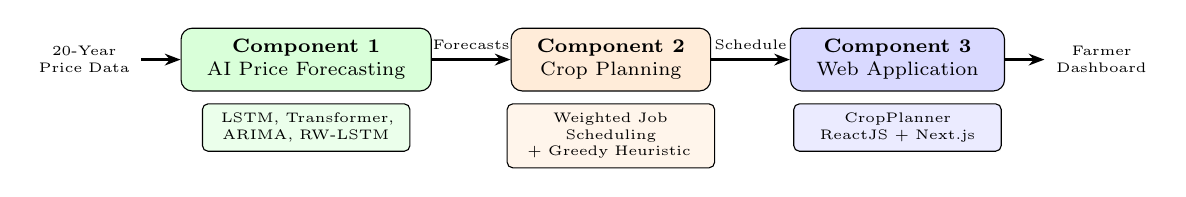
\begin{tikzpicture}[node distance=0.4cm]
    % Component 1
    \node[bigblock=green!15] (ai) {
      \begin{tabular}{c}
        \textbf{Component 1}\\
        AI Price Forecasting
      \end{tabular}
    };
    \node[smallblock=green!8, below=0.15cm of ai, text width=2.4cm, align=center] (aidet) {LSTM, Transformer,\\ARIMA, RW-LSTM};

    % Component 2
    \node[bigblock=orange!15, right=1.0cm of ai] (sched) {
      \begin{tabular}{c}
        \textbf{Component 2}\\
        Crop Planning
      \end{tabular}
    };
    \node[smallblock=orange!8, below=0.15cm of sched, text width=2.4cm, align=center] (scheddet) {Weighted Job Scheduling\\+ Greedy Heuristic};

    % Component 3
    \node[bigblock=blue!15, right=1.0cm of sched] (web) {
      \begin{tabular}{c}
        \textbf{Component 3}\\
        Web Application
      \end{tabular}
    };
    \node[smallblock=blue!8, below=0.15cm of web, text width=2.4cm, align=center] (webdet) {CropPlanner\\ReactJS + Next.js};

    % Arrows
    \draw[arrow] (ai) -- node[above, font=\tiny] {Forecasts} (sched);
    \draw[arrow] (sched) -- node[above, font=\tiny] {Schedule} (web);

    % Input/Output
    \node[left=0.5cm of ai, font=\tiny, text width=1.2cm, align=center] (input) {20-Year\\Price Data};
    \node[right=0.5cm of web, font=\tiny, text width=1.2cm, align=center] (output) {Farmer\\Dashboard};
    \draw[arrow] (input) -- (ai);
    \draw[arrow] (web) -- (output);
  \end{tikzpicture}}
  \caption{System overview of CropPlanner comprising three integrated components.}
  \label{fig:system}
\end{figure}

% ============================================================
% II. RELATED WORK
% ============================================================
\section{Related Work}
\label{sec:related}

\subsection{Time-Series Forecasting for Agricultural Prices}

Agricultural price forecasting has been extensively studied using statistical and machine learning approaches. Traditional ARIMA models~\cite{boxjenkins} remain widely used for linear time-series data but struggle with structural breaks and nonlinear patterns. Deep learning models have gained prominence, with LSTM networks---designed to capture long-term dependencies through gating mechanisms~\cite{hochreiter1997lstm}---and Transformer architectures---leveraging self-attention to process entire sequences simultaneously~\cite{vaswani2017attention}---showing superior performance on various forecasting benchmarks.

The relative merits of LSTM and Transformer models for commodity price forecasting remain an active research question. LSTM's inductive bias toward sequential processing makes it well-suited for short, univariate time series, while Transformers' global attention mechanism can capture long-range dependencies but may overfit on small datasets. Lim et al.~\cite{lim2021tft} introduced Temporal Fusion Transformers (TFT), which combine temporal attention with variable selection for multi-horizon forecasting, achieving state-of-the-art results on several benchmarks. Salinas et al.~\cite{salinas2020deepar} proposed DeepAR, an autoregressive recurrent model that produces probabilistic forecasts with prediction intervals---a feature absent from most agricultural forecasting studies. More recently, Zhou et al.~\cite{zhou2021informer} introduced Informer, which uses a ProbSparse self-attention mechanism to efficiently handle long sequence time-series forecasting, while Wu et al.~\cite{wu2021autoformer} proposed Autoformer with a decomposition-based architecture that separates trend and seasonal components within the Transformer framework.

A critical challenge in non-stationary price forecasting is concept drift---the distribution of price patterns shifts over time due to policy changes, supply shocks, and global economic cycles. Cerqueira et al.~\cite{cerqueira2020} conducted an empirical study on sliding-window and expanding-window evaluation strategies for time-series forecasting, finding that sliding windows better handle distributional shift by discarding outdated observations. This insight motivates our Rolling-Window LSTM approach, which restricts training to recent, more relevant data subsets.

Sabu and Kumar~\cite{rohan2025crop} demonstrated that LSTM models can significantly outperform ARIMA for agricultural commodity price prediction, achieving lower MAE on arecanut price forecasting. Javaid et al.~\cite{javaid2023ai} surveyed AI applications in agriculture broadly, including predictive analytics. However, most prior work forecasts a single crop in isolation and does not connect predictions to downstream planning systems.

\vfill
\newpage

\subsection{Crop Scheduling and Combinatorial Optimization}

Resource allocation in agriculture can be modeled as optimization problems such as the Knapsack Problem for area allocation or Job Scheduling for temporal planning. The Weighted Job Scheduling Problem (WJSP)---in which jobs have start times, end times, and weights (profits), and the goal is to select a maximum-weight subset of non-overlapping jobs---is a well-studied problem in combinatorial optimization. Cormen et al.~\cite{clrs2009} present the greedy approach for the unweighted variant, while Kleinberg and Tardos~\cite{kleinberg2005} provide the dynamic programming solution for the weighted case, achieving $O(n \log n)$ time complexity.

Sarker and Ray~\cite{sarker2009crop} formulated crop planning as a multi-objective optimization model and demonstrated the use of evolutionary algorithms to identify Pareto-optimal planting configurations that balance net return against crop diversity. Their work highlights the applicability of combinatorial optimization to agricultural scheduling, though it does not incorporate price forecasting as a decision input. Dury et al.~\cite{dury2012crop} surveyed models used to support cropping plan and crop rotation decisions, identifying three main approaches: rule-based, mathematical programming, and simulation-based models. Most rely on fixed agronomic calendars rather than dynamic price signals.

\subsection{Agricultural Decision Support Systems}

Agricultural Decision Support Systems (DSS) have been developed in various contexts. Zhai et al.~\cite{zhai2020dss} surveyed thirteen representative DSS for Agriculture~4.0, finding that most systems focus on individual sub-tasks---irrigation management, pest control, or nutrient planning---and typically rely on static agronomic data such as planting calendars or soil information rather than AI-driven price forecasts as decision variables. Gebbers and Adamchuk~\cite{gebbers2010} reviewed precision agriculture technologies, emphasizing the role of sensor data and spatial analysis in decision-making, but noted the limited integration of economic forecasting into farm management tools. Eli-Chukwu~\cite{elichukwu2019} surveyed applications of artificial intelligence in agriculture, identifying price prediction and crop recommendation as promising but underexplored areas for end-to-end system integration.

Table~\ref{tab:related_work} summarizes the key differences between representative prior works and the present study.

\begin{table*}[htbp]
  \centering
  \caption{Comparison of Related Work}
  \label{tab:related_work}
  \begin{tabular}{lcccccl}
    \toprule
    \textbf{Reference} & \textbf{Forecast Model} & \textbf{Crops} & \textbf{Scheduling} & \textbf{Web App} & \textbf{Peak Timing} & \textbf{Region} \\
    \midrule
    Sabu \& Kumar~\cite{rohan2025crop}      & LSTM, Trans.          & Single  & No  & No  & No  & General \\
    Lim et al.~\cite{lim2021tft}           & TFT                   & Multi   & No  & No  & No  & Multiple \\
    Salinas et al.~\cite{salinas2020deepar} & DeepAR                & Multi   & No  & No  & No  & Multiple \\
    Sarker \& Ray~\cite{sarker2009crop}     & None                  & Multi   & Evolutionary & No  & N/A & Australia \\
    Dury et al.~\cite{dury2012crop}         & None                  & Multi   & Survey       & No  & N/A & Europe \\
    Zhai et al.~\cite{zhai2020dss}          & Various               & Various & No           & Survey & No  & Global \\
    \midrule
    \textbf{This work} & \textbf{LSTM, Trans., ARIMA, RW-LSTM} & \textbf{4} & \textbf{WJSP + Greedy} & \textbf{Yes} & \textbf{Yes} & \textbf{Thailand} \\
    \bottomrule
  \end{tabular}
  \vspace{6pt}
  \par\raggedright\scriptsize\textit{Note:} ``Peak Timing'' indicates whether the work explicitly evaluates the accuracy of predicted peak price positions, distinct from overall forecast accuracy.
\end{table*}

The gap that this work addresses is the integration of AI price forecasting with scheduling optimization and farmer-accessible web delivery---a pipeline that has received limited attention in prior literature. To our knowledge, no prior study jointly evaluates multiple forecasting models on peak timing accuracy and uses the predicted peaks as inputs to a scheduling algorithm, while delivering results through an interactive web application.

% ============================================================
% III. DATA AND PREPROCESSING
% ============================================================
\newpage
\section{Data and Preprocessing}
\label{sec:data}

\subsection{Data Sources}

Price data were obtained from two Thai government agencies: the Department of Internal Trade (DIT) and the Office of Agricultural Economics (OAE). Table~\ref{tab:dataset} summarizes the dataset.

\begin{table}[htbp]
  \centering
  \caption{Dataset Summary}
  \label{tab:dataset}
  \begin{tabular}{ll}
    \toprule
    \textbf{Property} & \textbf{Value} \\
    \midrule
    Crops & Cassava, Corn, Green Bean, Soybean \\
    Region & Northeastern Thailand \\
    Period & Jan 2004 -- Dec 2024 (20 years) \\
    Frequency & Monthly \\
    Records & $\sim$252 per crop \\
    Currency & Thai Baht (THB/kg) \\
    \bottomrule
  \end{tabular}
\end{table}

\subsection{Preprocessing}

Raw data in PDF and Excel format with Thai Buddhist Era dates underwent several cleaning steps: date conversion from Buddhist Era (BE) to Common Era (CE), duplicate removal, and unit normalization. Processing was performed using Python with Pandas and NumPy. The final cleaned data was stored in long-format CSV files with \texttt{date} and \texttt{price} columns.

\begin{figure}[htbp]
  \centering
  \resizebox{\columnwidth}{!}{%
  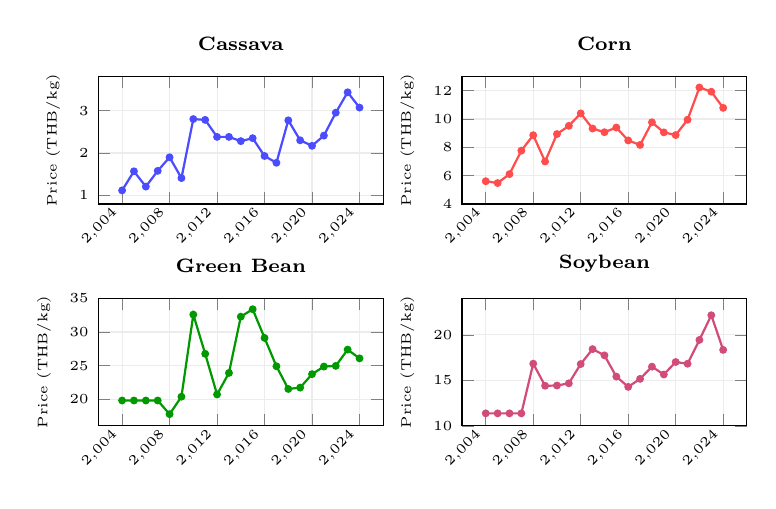
\begin{tikzpicture}
    \begin{groupplot}[
      group style={group size=2 by 2, horizontal sep=1cm, vertical sep=1.2cm},
      width=5.2cm, height=3.2cm,
      ylabel={Price (THB/kg)},
      ylabel style={font=\tiny},
      xticklabel style={font=\tiny, rotate=45, anchor=east},
      yticklabel style={font=\tiny},
      title style={font=\scriptsize\bfseries},
      grid=major, grid style={gray!15},
      xtick={2004,2008,2012,2016,2020,2024},
      every axis plot/.append style={mark size=1pt, thick},
    ]
    \nextgroupplot[title={Cassava}, ymin=0.8, ymax=3.8]
    \addplot[blue!70, mark=*, mark options={fill=blue!70}] coordinates {
      (2004,1.12)(2005,1.57)(2006,1.21)(2007,1.58)(2008,1.90)(2009,1.41)(2010,2.80)
      (2011,2.78)(2012,2.38)(2013,2.38)(2014,2.28)(2015,2.35)(2016,1.93)(2017,1.77)
      (2018,2.77)(2019,2.30)(2020,2.17)(2021,2.41)(2022,2.95)(2023,3.43)(2024,3.07)
    };
    \nextgroupplot[title={Corn}, ymin=4, ymax=13]
    \addplot[red!70, mark=*, mark options={fill=red!70}] coordinates {
      (2004,5.61)(2005,5.48)(2006,6.11)(2007,7.77)(2008,8.86)(2009,7.00)(2010,8.94)
      (2011,9.52)(2012,10.40)(2013,9.33)(2014,9.07)(2015,9.40)(2016,8.49)(2017,8.17)
      (2018,9.77)(2019,9.06)(2020,8.87)(2021,9.95)(2022,12.23)(2023,11.93)(2024,10.79)
    };
    \nextgroupplot[title={Green Bean}, ymin=16, ymax=35]
    \addplot[green!60!black, mark=*, mark options={fill=green!60!black}] coordinates {
      (2004,19.79)(2005,19.79)(2006,19.79)(2007,19.79)(2008,17.75)(2009,20.36)(2010,32.60)
      (2011,26.75)(2012,20.69)(2013,23.90)(2014,32.29)(2015,33.40)(2016,29.12)(2017,24.90)
      (2018,21.51)(2019,21.71)(2020,23.72)(2021,24.85)(2022,24.95)(2023,27.38)(2024,26.07)
    };
    \nextgroupplot[title={Soybean}, ymin=10, ymax=24]
    \addplot[purple!70, mark=*, mark options={fill=purple!70}] coordinates {
      (2004,11.38)(2005,11.38)(2006,11.38)(2007,11.38)(2008,16.84)(2009,14.41)(2010,14.44)
      (2011,14.68)(2012,16.80)(2013,18.44)(2014,17.75)(2015,15.42)(2016,14.29)(2017,15.17)
      (2018,16.51)(2019,15.65)(2020,17.02)(2021,16.83)(2022,19.45)(2023,22.16)(2024,18.35)
    };
    \end{groupplot}
  \end{tikzpicture}}%
  \caption{Yearly average prices (2004--2024) for four Thai field crops showing long-term trends, structural breaks, and the distinct price scales of each commodity.}
  \label{fig:trends}
\end{figure}

\subsection{Descriptive Statistics}

Table~\ref{tab:descriptive} summarizes the key statistical properties of each crop's price series. The four crops span distinct price ranges---from cassava at 1--4~THB/kg to green bean at 17--34~THB/kg---and exhibit different volatility profiles.

\begin{table}[htbp]
  \centering
  \caption{Descriptive Statistics of Yearly Average Prices (2004--2024)}
  \label{tab:descriptive}
  \begin{tabular}{lccccc}
    \toprule
    \textbf{Crop} & \textbf{Mean} & \textbf{Min} & \textbf{Max} & \textbf{YoY Std} & \textbf{Trend} \\
    & (THB/kg) & (THB/kg) & (THB/kg) & (\%) & (\%) \\
    \midrule
    Cassava    & 2.22 & 1.12 & 3.43 & 30.4 & $+$174 \\
    Corn       & 8.89 & 5.48 & 12.23 & 13.6 & $+$92 \\
    Green Bean & 24.34 & 17.75 & 33.40 & 19.0 & $+$32 \\
    Soybean    & 15.70 & 11.38 & 22.16 & 14.1 & $+$61 \\
    \bottomrule
  \end{tabular}
  \vspace{6pt}
  \par\raggedright\scriptsize\textit{Note:} ``YoY Std'' is the standard deviation of year-over-year percentage changes. ``Trend'' is the overall percentage change from 2004 to 2024.
\end{table}

Cassava exhibits the highest volatility (YoY~Std~=~30.4\%) with three extreme years: 2005 (+40\%), 2010 (+99\%), and 2018 (+57\%). This high volatility, combined with its long growing period (250~days), makes cassava particularly challenging to forecast and schedule. Corn shows more moderate but consistent growth (+92\% over 20~years), with 5~high-volatility years. Green bean and soybean display lower long-term trends but exhibit significant seasonal variation within each year, which is more relevant for the monthly forecasting task.

Autocorrelation analysis of the monthly price series reveals strong persistence at short lags (lag-1 autocorrelation $> 0.9$ for all crops) and significant seasonal patterns at lag~12, confirming that recent prices are highly predictive of near-term behavior. This motivates the use of sequence models (LSTM, Transformer) that can learn temporal dependencies. The lag-12 significance also supports the ARIMA model's seasonal component, though the non-stationarity identified in Section~\ref{sec:limitations} limits ARIMA's effectiveness for crops with structural breaks.

Fig.~\ref{fig:seasonal} illustrates the contrast between two crops via additive seasonal decomposition (12-month moving average, 2015--2024). Cassava's trend component exhibits sharp directional changes---a decline from 2016 to 2017, a spike in 2018, and a sustained rise from 2021---reflecting the structural breaks that challenge ARIMA's stationarity assumption. Its seasonal component is weak (amplitude $\approx \pm 0.08$~THB/kg), meaning price movements are driven primarily by trend and residual shocks rather than periodic patterns. Green bean, in contrast, shows a more stable trend but a pronounced seasonal component (amplitude $\approx \pm 1.3$~THB/kg) with peaks in months~2 and~5 and troughs in months~7 and~11, providing the regular periodicity that ARIMA can capture effectively.

% --- Fig: Seasonal Decomposition ---
\begin{figure*}[htbp]
  \centering
  \resizebox{\textwidth}{!}{%
  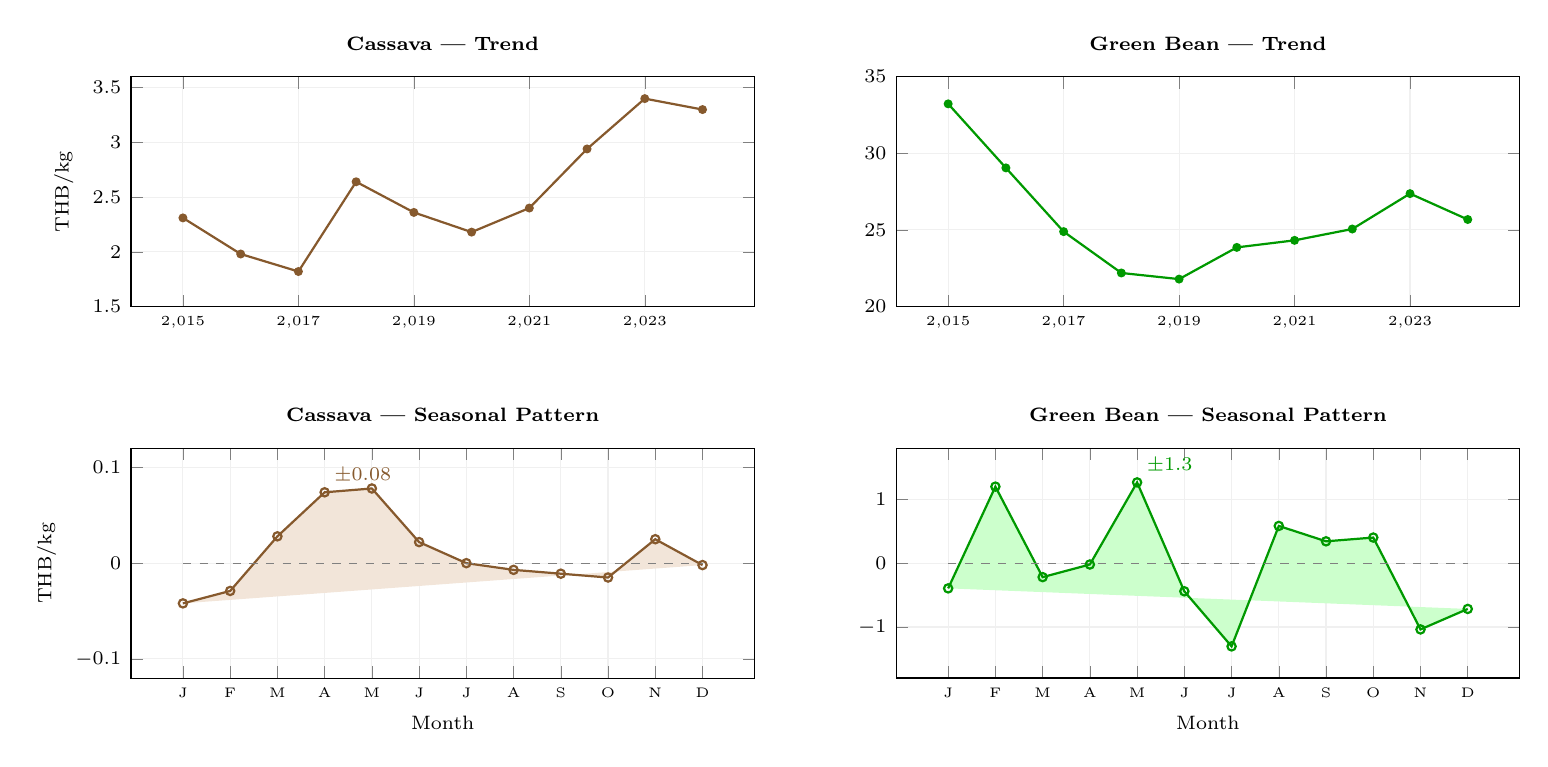
\begin{tikzpicture}
    \begin{groupplot}[
      group style={group size=2 by 2, horizontal sep=1.8cm, vertical sep=1.8cm},
      width=9.5cm, height=4.5cm,
      xlabel style={font=\scriptsize},
      ylabel style={font=\scriptsize},
      xticklabel style={font=\tiny},
      yticklabel style={font=\scriptsize},
      title style={font=\scriptsize\bfseries},
      grid=major, grid style={gray!12},
      every axis plot/.append style={thick},
    ]

    % === Cassava Trend ===
    \nextgroupplot[
      title={Cassava --- Trend},
      ylabel={\scriptsize THB/kg},
      xtick={2015,2017,2019,2021,2023},
      ymin=1.5, ymax=3.6,
    ]
    \addplot[brown!70!black, mark=*, mark size=1.2pt] coordinates {
      (2015,2.31)(2016,1.98)(2017,1.82)(2018,2.64)(2019,2.36)
      (2020,2.18)(2021,2.40)(2022,2.94)(2023,3.40)(2024,3.30)
    };

    % === Green Bean Trend ===
    \nextgroupplot[
      title={Green Bean --- Trend},
      xtick={2015,2017,2019,2021,2023},
      ymin=20, ymax=35,
    ]
    \addplot[green!60!black, mark=*, mark size=1.2pt] coordinates {
      (2015,33.23)(2016,29.05)(2017,24.89)(2018,22.19)(2019,21.79)
      (2020,23.86)(2021,24.32)(2022,25.06)(2023,27.37)(2024,25.68)
    };

    % === Cassava Seasonal ===
    \nextgroupplot[
      title={Cassava --- Seasonal Pattern},
      ylabel={\scriptsize THB/kg},
      xlabel={\scriptsize Month},
      xtick={1,2,...,12},
      xticklabels={J,F,M,A,M,J,J,A,S,O,N,D},
      ymin=-0.12, ymax=0.12,
    ]
    \addplot[brown!70!black, thick, mark=o, mark size=1.5pt, fill=brown!20] coordinates {
      (1,-0.042)(2,-0.029)(3,0.028)(4,0.074)(5,0.078)(6,0.022)
      (7,0.000)(8,-0.007)(9,-0.011)(10,-0.015)(11,0.025)(12,-0.002)
    };
    \addplot[gray, dashed, thin] coordinates {(1,0)(12,0)};
    \node[font=\tiny, brown!70!black, above right] at (axis cs:4,0.074) {\scriptsize $\pm$0.08};

    % === Green Bean Seasonal ===
    \nextgroupplot[
      title={Green Bean --- Seasonal Pattern},
      xlabel={\scriptsize Month},
      xtick={1,2,...,12},
      xticklabels={J,F,M,A,M,J,J,A,S,O,N,D},
      ymin=-1.8, ymax=1.8,
    ]
    \addplot[green!60!black, thick, mark=o, mark size=1.5pt, fill=green!20] coordinates {
      (1,-0.395)(2,1.199)(3,-0.219)(4,-0.021)(5,1.265)(6,-0.441)
      (7,-1.304)(8,0.583)(9,0.342)(10,0.401)(11,-1.038)(12,-0.717)
    };
    \addplot[gray, dashed, thin] coordinates {(1,0)(12,0)};
    \node[font=\tiny, green!60!black, above right] at (axis cs:5,1.265) {\scriptsize $\pm$1.3};

    \end{groupplot}
  \end{tikzpicture}}%
  \caption{Seasonal decomposition comparison (2015--2024). \textbf{Top row:} yearly trend (12-month moving average). Cassava shows sharp structural breaks (2017 trough, 2018 spike); green bean shows a smoother U-shaped trend. \textbf{Bottom row:} average monthly seasonal deviation. Cassava's seasonal component is negligible ($\pm$0.08~THB/kg); green bean exhibits clear seasonality ($\pm$1.3~THB/kg) with peaks in Feb and May.}
  \label{fig:seasonal}
\end{figure*}

\subsection{Train--Validation--Test Split}

Data were divided into three partitions: a training set (2004--2022), a validation set (2023), and a test set (2024). The scaler was fit exclusively on training data to prevent data leakage. The validation set was used solely for hyperparameter selection---specifically, the Rolling-Window LSTM window size (Section~\ref{sec:rwlstm})---ensuring that the test set remained entirely unseen during model development. For the final evaluation, models were retrained on the combined training and validation data (2004--2023) and evaluated on the held-out test year (2024).


% ============================================================
% IV. METHODOLOGY
% ============================================================
\section{Methodology}
\label{sec:methodology}

The CropPlanner system comprises three components: (A)~AI~price forecasting models, (B)~crop planning recommendation, and (C)~a~web application. All models take 12~months of historical prices as input and produce 12-month forecasts.

\subsection{AI Price Forecasting Models}

Table~\ref{tab:hyperparams} summarizes the hyperparameters of all four models.

\begin{table}[htbp]
  \centering
  \caption{Hyperparameter Summary}
  \label{tab:hyperparams}
  \begin{tabular}{lcccc}
    \toprule
    \textbf{Parameter} & \textbf{LSTM} & \textbf{Trans.} & \textbf{ARIMA} & \textbf{RW-LSTM} \\
    \midrule
    Architecture & 2-layer & 2-layer enc. & Auto & 3-layer \\
    Hidden / $d_{\text{model}}$ & 32 & 64 & auto & 32 \\
    Attn.\ heads & -- & 8 & -- & -- \\
    FF dim & -- & 128 & -- & -- \\
    Epochs & 300 & 500 & -- & 300 \\
    Learning rate & 0.01 & 0.001 & -- & 0.01 \\
    Loss function & MSE & MSE & -- & MSE \\
    Library & PyTorch & PyTorch & StatsFC & PyTorch \\
    \bottomrule
  \end{tabular}
\end{table}

\subsubsection{Standard LSTM}

Long Short-Term Memory (LSTM)~\cite{hochreiter1997lstm} is a recurrent neural network designed to learn long-term dependencies via gating mechanisms (forget, input, and output gates). Our model consists of 2~layers with hidden size~32, receiving 12~months of input and producing 12~months of output.

All input prices are normalized using MinMaxScaler fitted exclusively on training data to prevent information leakage. The model is trained using Mean Squared Error (MSE) loss with the Adam optimizer (learning rate $= 0.01$) for a fixed 300~epochs. Full-batch training is employed---the entire training set is passed as a single batch per epoch---which stabilizes gradient estimation given the small dataset size ($\sim$228 samples after windowing). No learning rate scheduling or early stopping is applied; instead, the fixed epoch budget and small model capacity (2,080 parameters) serve as implicit regularization. All experiments use a fixed random seed of~42 for reproducibility.

% --- Fig. 3: LSTM Architecture (from code: lstm_model.py) ---
\begin{figure}[htbp]
  \centering
  \resizebox{\columnwidth}{!}{%
  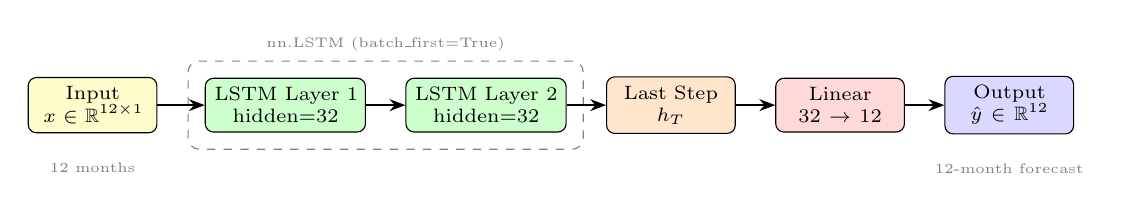
\begin{tikzpicture}[node distance=0.35cm and 0.3cm]
    % Input
    \node[block=yellow!20, text width=1.4cm, align=center] (input) {Input\\$x \in \mathbb{R}^{12 \times 1}$};

    % LSTM layers
    \node[block=green!20, right=0.6cm of input, text width=1.8cm, align=center] (lstm1) {LSTM Layer 1\\hidden=32};
    \node[block=green!20, right=0.5cm of lstm1, text width=1.8cm, align=center] (lstm2) {LSTM Layer 2\\hidden=32};

    % Last hidden state
    \node[block=orange!20, right=0.5cm of lstm2, text width=1.4cm, align=center] (last) {Last Step\\$h_{T}$};

    % FC
    \node[block=red!15, right=0.5cm of last, text width=1.4cm, align=center] (fc) {Linear\\$32 \to 12$};

    % Output
    \node[block=blue!15, right=0.5cm of fc, text width=1.4cm, align=center] (output) {Output\\$\hat{y} \in \mathbb{R}^{12}$};

    % Arrows
    \draw[arrow] (input) -- (lstm1);
    \draw[arrow] (lstm1) -- (lstm2);
    \draw[arrow] (lstm2) -- (last);
    \draw[arrow] (last) -- (fc);
    \draw[arrow] (fc) -- (output);

    % Annotations
    \node[below=0.25cm of input, font=\tiny, text=gray] {12 months};
    \node[below=0.25cm of output, font=\tiny, text=gray] {12-month forecast};

    % Group LSTM
    \begin{scope}[on background layer]
      \node[group, fit=(lstm1)(lstm2), label={[font=\tiny, text=gray]above:nn.LSTM (batch\_first=True)}] {};
    \end{scope}
  \end{tikzpicture}}
  \caption{Standard LSTM architecture. Input sequence of 12 monthly prices passes through 2~LSTM layers (hidden=32). The last time step's hidden state is projected to 12 output values via a linear layer.}
  \label{fig:lstm}
\end{figure}

\subsubsection{Transformer}

The Transformer model~\cite{vaswani2017attention} uses multi-head self-attention to process the entire sequence simultaneously, efficiently capturing global dependencies across time steps. We adopt an encoder-only architecture rather than the full encoder--decoder design because our task is direct multi-step regression (12~inputs $\to$ 12~outputs via a linear head), not autoregressive sequence generation. Scalar monthly prices are first projected to the model dimension via a learned linear layer ($1 \to d_{\text{model}} = 64$), then augmented with sinusoidal positional encoding to preserve temporal ordering. The encoder consists of 2~layers, each with 8-head self-attention and a feed-forward network ($d_{ff} = 128$). The last time step's hidden representation is extracted and projected to 12~output values via a linear layer. Training uses MSE loss with the Adam optimizer (learning rate $= 0.001$) for 500~epochs, with the same MinMaxScaler preprocessing and full-batch training protocol as LSTM.

% --- Fig. 4: Transformer Architecture (from code: transformer_model.py) ---
\begin{figure}[htbp]
  \centering
  \resizebox{\columnwidth}{!}{%
  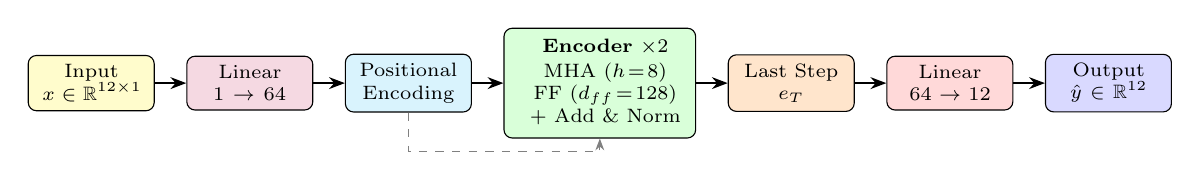
\begin{tikzpicture}[node distance=0.35cm and 0.4cm]
    % Input
    \node[block=yellow!20, text width=1.3cm, align=center] (input) {Input\\$x \in \mathbb{R}^{12 \times 1}$};

    % Input projection
    \node[block=purple!15, right=0.4cm of input, text width=1.3cm, align=center] (proj) {Linear\\$1 \to 64$};

    % Positional Encoding
    \node[block=cyan!15, right=0.4cm of proj, text width=1.3cm, align=center] (pe) {Positional\\Encoding};

    % Encoder block (repeated)
    \node[block=green!15, right=0.4cm of pe, text width=2.2cm, align=center, minimum height=1.2cm] (enc) {
      \begin{tabular}{c}
        \textbf{Encoder} $\times 2$\\[1pt]
        MHA ($h\!=\!8$)\\
        FF ($d_{ff}\!=\!128$)\\
        + Add \& Norm
      \end{tabular}
    };

    % Last step
    \node[block=orange!20, right=0.4cm of enc, text width=1.2cm, align=center] (last) {Last Step\\$e_{T}$};

    % Decoder
    \node[block=red!15, right=0.4cm of last, text width=1.2cm, align=center] (dec) {Linear\\$64 \to 12$};

    % Output
    \node[block=blue!15, right=0.4cm of dec, text width=1.3cm, align=center] (output) {Output\\$\hat{y} \in \mathbb{R}^{12}$};

    % Arrows
    \draw[arrow] (input) -- (proj);
    \draw[arrow] (proj) -- (pe);
    \draw[arrow] (pe) -- (enc);
    \draw[arrow] (enc) -- (last);
    \draw[arrow] (last) -- (dec);
    \draw[arrow] (dec) -- (output);

    % Add + residual annotation
    \draw[-{Stealth[length=1.5mm]}, gray, dashed] (pe.south) -- ++(0,-0.5) -| (enc.south);
  \end{tikzpicture}}%
  \caption{Transformer architecture (encoder-only). Prices are projected to $d_{\text{model}}=64$, augmented with positional encoding, and processed by 2~encoder layers with 8-head attention. The last time step's hidden representation is projected to 12~output values via a linear layer.}
  \label{fig:transformer}
\end{figure}

\subsubsection{ARIMA}

ARIMA (Autoregressive Integrated Moving Average)~\cite{boxjenkins} combines autoregressive, differencing, and moving average components. We use AutoARIMA from the StatsForecast library with \texttt{season\_length}$= 12$ and stepwise search, which automatically selects optimal $(p, d, q)$ parameters through time-series decomposition into trend, seasonality, and residual components.

Prior to model fitting, Augmented Dickey--Fuller (ADF) tests were applied to the training data for each crop. Cassava and corn exhibited non-stationarity ($p > 0.05$), requiring first-order differencing ($d = 1$). Green bean and soybean were borderline stationary, and AutoARIMA selected $d = 0$ or $d = 1$ depending on the specific window. Unlike the deep learning models, ARIMA requires no manual hyperparameter specification---the $(p, d, q)$ orders are determined entirely by the automated selection procedure, and results are cached for reproducibility.

% --- Fig. 5: ARIMA Pipeline ---
\begin{figure}[htbp]
  \centering
  \resizebox{\columnwidth}{!}{%
  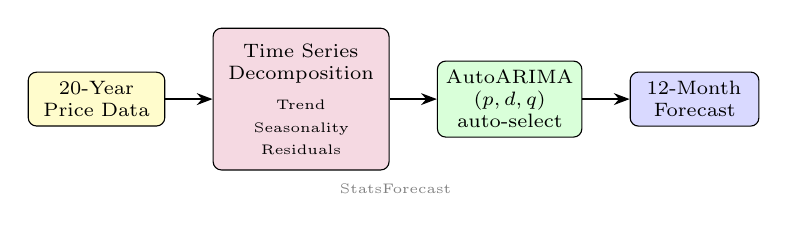
\begin{tikzpicture}[node distance=0.4cm]
    % Data
    \node[block=yellow!20, text width=1.5cm, align=center] (data) {20-Year\\Price Data};

    % Decomposition
    \node[block=purple!15, right=0.6cm of data, text width=2.0cm, align=center, minimum height=1.8cm] (decomp) {Time Series\\Decomposition\\[3pt]{\tiny Trend}\\{\tiny Seasonality}\\{\tiny Residuals}};

    % AutoARIMA
    \node[block=green!15, right=0.6cm of decomp, text width=1.6cm, align=center] (arima) {AutoARIMA\\$(p,d,q)$\\auto-select};

    % Output
    \node[block=blue!15, right=0.6cm of arima, text width=1.4cm, align=center] (out) {12-Month\\Forecast};

    % Arrows
    \draw[arrow] (data) -- (decomp);
    \draw[arrow] (decomp) -- (arima);
    \draw[arrow] (arima) -- (out);

    % StatsForecast label centered under entire pipeline
    \node[below=0.6cm of $(data.south)!0.5!(out.south)$, font=\tiny, text=gray] {StatsForecast};
  \end{tikzpicture}}
  \caption{ARIMA forecasting pipeline. Historical data is decomposed into trend, seasonality, and residual components before AutoARIMA selects optimal $(p,d,q)$ parameters.}
  \label{fig:arima}
\end{figure}

\subsubsection{Limitations of Standard Models}
\label{sec:limitations}

Before presenting our proposed improvement, we first establish the limitations of the standard models that motivate it. Analysis of Standard LSTM and Transformer predictions on the 2024 test year reveals three systematic issues when these models are trained on the full 20-year historical period.

\textit{Issue~1: Off-Peak Prediction.} The Standard LSTM produces smooth, gradually varying curves that fail to capture sharp seasonal price spikes. Fig.~\ref{fig:lstm_gb_limit} illustrates this for green bean: the actual price peaks sharply at 31.00~THB/kg in September, while the LSTM predicts a gradual bell curve peaking in July at 26.83~THB/kg---a peak timing error of 2~months. Fig.~\ref{fig:lstm_corn_limit} shows a more severe case for corn: the actual price exhibits a pronounced June--July spike to 12.45~THB/kg, while the LSTM predicts a nearly flat curve ranging from 10.43 to 10.82~THB/kg, with a peak timing error of 4~months (predicted March vs.\ actual July) and 15.46\% error at the actual peak month. This ``smoothing effect'' arises because the model averages across 20~years of diverse seasonal patterns, producing predictions that resemble the long-run mean rather than the sharp, year-specific peaks that matter for scheduling.

% --- Fig: Green Bean Standard LSTM Limitation ---
\begin{figure}[htbp]
  \centering
  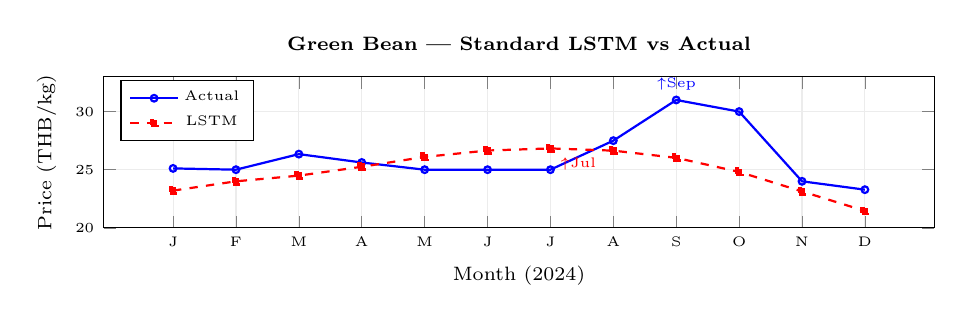
\begin{tikzpicture}
    \begin{axis}[
      width=\columnwidth, height=3.5cm,
      xlabel={\scriptsize Month (2024)}, ylabel={\scriptsize Price (THB/kg)},
      xticklabel style={font=\tiny}, yticklabel style={font=\tiny},
      xlabel style={font=\tiny}, ylabel style={font=\tiny},
      title={\scriptsize\bfseries Green Bean --- Standard LSTM vs Actual},
      xtick={1,2,...,12},
      xticklabels={J,F,M,A,M,J,J,A,S,O,N,D},
      ymin=20, ymax=33, grid=major, grid style={gray!15},
      legend style={font=\tiny, at={(0.02,0.98)}, anchor=north west},
    ]
    \addplot[blue, thick, mark=o, mark size=1.2pt] coordinates {
      (1,25.11)(2,25.00)(3,26.34)(4,25.62)(5,25.00)(6,25.00)
      (7,25.00)(8,27.50)(9,31.00)(10,30.00)(11,24.00)(12,23.28)
    }; \addlegendentry{Actual}
    \addplot[red, dashed, thick, mark=square*, mark size=1.2pt] coordinates {
      (1,23.20)(2,24.00)(3,24.49)(4,25.25)(5,26.10)(6,26.65)
      (7,26.83)(8,26.64)(9,26.02)(10,24.81)(11,23.13)(12,21.45)
    }; \addlegendentry{LSTM}
    % Peak markers
    \node[font=\tiny, blue, above] at (axis cs:9,31.00) {$\uparrow$Sep};
    \node[font=\tiny, red, below right] at (axis cs:7,26.83) {$\uparrow$Jul};
    \end{axis}
  \end{tikzpicture}
  \caption{Green bean 2024: Standard LSTM produces a smooth bell curve peaking in Jul, missing the sharp Sep peak entirely ($\Delta$Month~=~2).}
  \label{fig:lstm_gb_limit}
\end{figure}

% --- Fig: Corn Standard LSTM Limitation ---
\begin{figure}[htbp]
  \centering
  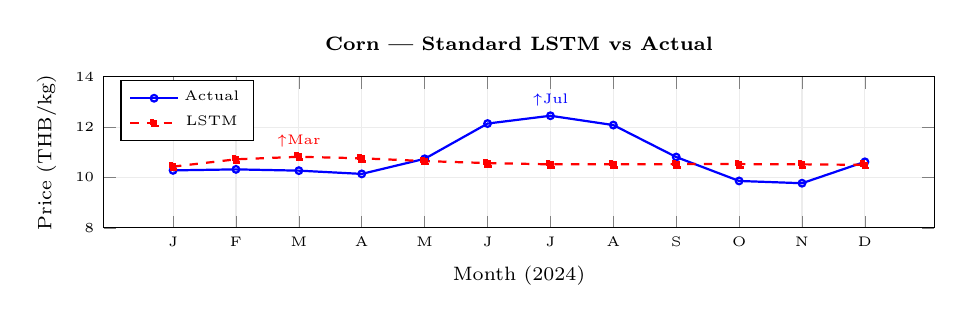
\begin{tikzpicture}
    \begin{axis}[
      width=\columnwidth, height=3.5cm,
      xlabel={\scriptsize Month (2024)}, ylabel={\scriptsize Price (THB/kg)},
      xticklabel style={font=\tiny}, yticklabel style={font=\tiny},
      xlabel style={font=\tiny}, ylabel style={font=\tiny},
      title={\scriptsize\bfseries Corn --- Standard LSTM vs Actual},
      xtick={1,2,...,12},
      xticklabels={J,F,M,A,M,J,J,A,S,O,N,D},
      ymin=8, ymax=14, grid=major, grid style={gray!15},
      legend style={font=\tiny, at={(0.02,0.98)}, anchor=north west},
    ]
    \addplot[blue, thick, mark=o, mark size=1.2pt] coordinates {
      (1,10.28)(2,10.32)(3,10.27)(4,10.14)(5,10.74)(6,12.14)
      (7,12.45)(8,12.08)(9,10.81)(10,9.86)(11,9.77)(12,10.62)
    }; \addlegendentry{Actual}
    \addplot[red, dashed, thick, mark=square*, mark size=1.2pt] coordinates {
      (1,10.43)(2,10.72)(3,10.82)(4,10.76)(5,10.65)(6,10.57)
      (7,10.52)(8,10.52)(9,10.53)(10,10.53)(11,10.52)(12,10.50)
    }; \addlegendentry{LSTM}
    % Peak markers
    \node[font=\tiny, blue, above] at (axis cs:7,12.45) {$\uparrow$Jul};
    \node[font=\tiny, red, above] at (axis cs:3,10.82) {$\uparrow$Mar};
    \end{axis}
  \end{tikzpicture}
  \caption{Corn 2024: Standard LSTM predicts a nearly flat curve (range 10.43--10.82) that completely misses the Jun--Jul price spike to 12.45~THB/kg ($\Delta$Month~=~4, peak error~=~15.46\%).}
  \label{fig:lstm_corn_limit}
\end{figure}

\textit{Issue~2: Long-Range Averaging.} With 252~data points spanning 20~years, the models are exposed to structurally different economic eras. Agricultural prices before 2010 were influenced by different policy regimes, supply chains, and global commodity cycles than those after 2018. The 2008 global financial crisis caused soybean prices to spike 48\% year-over-year, while the 2010 Thai floods triggered a 99\% surge in cassava prices. Training on the entire period forces the model to average across these regimes, diluting the representation of recent seasonal patterns that are most predictive of near-term behavior.

\textit{Issue~3: Structural Break Sensitivity.} The yearly trend analysis (Fig.~\ref{fig:trends}) reveals multiple structural breaks across the 20-year period: (i)~the 2008 global financial crisis, (ii)~the 2010 flood-driven commodity shock, (iii)~the 2014 policy shift affecting green bean prices (+35\% year-over-year), and (iv)~the 2022 post-COVID commodity boom. These breaks violate the stationarity assumptions underlying both ARIMA (explicitly) and the implicit assumption of deep learning models that training and test distributions are similar. ARIMA's poor performance on cassava (MAPE~=~24.71\%) is directly attributable to its stationarity requirement being violated by these structural breaks.

These three limitations---off-peak prediction, long-range averaging, and structural break sensitivity---motivate a windowed approach that learns from shorter, more recent data subsets, as described in the following section.

\subsubsection{Rolling-Window LSTM (Proposed Improvement)}
\label{sec:rwlstm}

To address the limitations identified in Section~\ref{sec:limitations}, we propose the Rolling-Window LSTM. The key insight is that shorter training windows reduce the influence of structurally different early periods, allowing the model to focus on recent seasonal patterns that better predict near-term price behavior. However, shorter windows also reduce training data volume, creating a bias--variance trade-off that must be resolved empirically via validation.

% --- Fig. 6: Rolling-Window Concept ---
\begin{figure}[htbp]
  \centering
  \resizebox{\columnwidth}{!}{%
  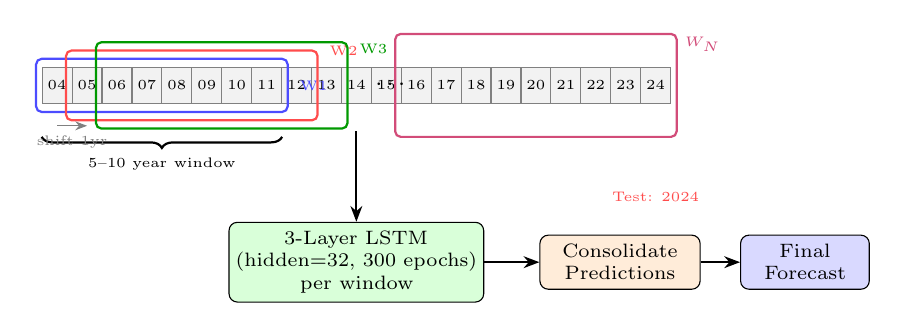
\begin{tikzpicture}[
    yearbox/.style={rectangle, minimum width=0.38cm, minimum height=0.45cm, draw=black!50, font=\tiny, inner sep=1pt},
    winbrace/.style={decorate, decoration={brace, amplitude=4pt, mirror}, thick}
  ]
    % Year boxes
    \foreach \i/\yr in {0/04,1/05,2/06,3/07,4/08,5/09,6/10,7/11,8/12,9/13,10/14,11/15,12/16,13/17,14/18,15/19,16/20,17/21,18/22,19/23,20/24} {
      \node[yearbox, fill=gray!10] (y\i) at (\i*0.38, 0) {\yr};
    }

    % Window 1 (8-year example)
    \draw[thick, blue!70, rounded corners=2pt] ([xshift=-2pt, yshift=3pt]y0.north west) rectangle ([xshift=2pt, yshift=-3pt]y7.south east);
    \node[right=0.1cm of y7, font=\tiny, blue!70] {W1};

    % Window 2
    \draw[thick, red!70, rounded corners=2pt] ([xshift=-2pt, yshift=6pt]y1.north west) rectangle ([xshift=2pt, yshift=-6pt]y8.south east);
    \node[above right=0.02cm and 0.1cm of y8, font=\tiny, red!70] {W2};

    % Window 3
    \draw[thick, green!60!black, rounded corners=2pt] ([xshift=-2pt, yshift=9pt]y2.north west) rectangle ([xshift=2pt, yshift=-9pt]y9.south east);
    \node[above right=0.05cm and 0.1cm of y9, font=\tiny, green!60!black] {W3};

    % Dots
    \node[right=0.3cm of y9, font=\small] (dots) {$\cdots$};

    % Last window
    \draw[thick, purple!70, rounded corners=2pt] ([xshift=-2pt, yshift=12pt]y12.north west) rectangle ([xshift=2pt, yshift=-12pt]y20.south east);
    \node[above right=0.08cm and 0.05cm of y20, font=\tiny, purple!70] {$W_N$};

    % Shift annotation
    \draw[winbrace] ([yshift=-12pt]y0.south west) -- node[below=4pt, font=\tiny] {5--10 year window} ([yshift=-12pt]y7.south east);

    % Arrow showing shift
    \draw[-{Stealth[length=1.5mm]}, gray] ([yshift=-8pt]y0.south) -- node[below, font=\tiny] {shift 1yr} ([yshift=-8pt]y1.south);

    % Target year
    \node[below=1.0cm of y20, font=\tiny, text=red!70] {Test: 2024};

    % LSTM box below
    \node[block=green!15, below=1.5cm of y10, text width=3cm, align=center] (lstm3) {3-Layer LSTM\\(hidden=32, 300 epochs)\\per window};

    % Consolidate
    \node[block=orange!15, right=0.7cm of lstm3, text width=1.8cm, align=center] (consol) {Consolidate\\Predictions};

    \node[block=blue!15, right=0.5cm of consol, text width=1.4cm, align=center] (final) {Final\\Forecast};

    \draw[arrow] ([yshift=-10pt]y10.south) -- (lstm3);
    \draw[arrow] (lstm3) -- (consol);
    \draw[arrow] (consol) -- (final);
  \end{tikzpicture}}%
  \caption{Rolling-Window LSTM training concept. The dataset is divided into overlapping windows of 5--10~years (selected per crop via validation), each shifted by 1~year. A 3-layer LSTM is trained on each window independently; predictions are consolidated into a final forecast.}
  \label{fig:rolling}
\end{figure}

The dataset is divided into candidate windows of 5--10~years (crop-dependent, selected via validation), each shifted by 1~year. For each candidate window size, a~3-layer LSTM (hidden size~32, 300~epochs) is trained on the corresponding training window and evaluated on the 2023 validation year. The window size yielding the lowest validation MAPE is selected, and the final model is trained on a single window of that size ending at the last available training year (Algorithm~\ref{alg:rwlstm}). Importantly, the ``consolidation'' step in the final model is trivial: only one window (the best-validated size) produces the final forecast. The rolling aspect is used during the validation sweep to evaluate multiple window sizes, not to average across windows at inference time.

Window sizes were selected via validation-set evaluation. For each crop, we swept window sizes from 5 to 10~years and selected the size yielding the lowest MAPE on the 2023 validation year. Table~\ref{tab:window_selection} presents the validation results. Cassava achieved the best validation MAPE with an 8-year window (31.25\%), corn with a 6-year window (11.43\%), while green bean and soybean performed best with 5-year windows (12.67\% and 15.62\%, respectively). The final models were then retrained on the combined training and validation data (2004--2023) using these selected window sizes and evaluated on the held-out test year (2024). By learning from shorter, more recent windows, the model avoids the long-range averaging problem (Section~\ref{sec:limitations}) and captures recent seasonal patterns more accurately---particularly the location of peak prices, which is critical for the downstream scheduling system.

\begin{table}[htbp]
  \centering
  \caption{Validation MAPE (\%) by Window Size (Year 2023)}
  \label{tab:window_selection}
  \begin{tabular}{lcccccc}
    \toprule
    \textbf{Crop} & \textbf{5yr} & \textbf{6yr} & \textbf{7yr} & \textbf{8yr} & \textbf{9yr} & \textbf{10yr} \\
    \midrule
    Cassava    & 35.09 & 31.31 & 33.15 & \textbf{31.25} & 31.53 & 32.03 \\
    Corn       & 13.08 & \textbf{11.43} & 14.23 & 11.44 & 13.60 & 20.27 \\
    Green Bean & \textbf{12.67} & 13.34 & 16.20 & 14.39 & 14.96 & 21.47 \\
    Soybean    & \textbf{15.62} & 20.48 & 19.15 & 23.72 & 25.07 & 21.73 \\
    \bottomrule
  \end{tabular}
  \vspace{6pt}
  \par\raggedright\scriptsize\textit{Note:} Bold values indicate the selected window size per crop (lowest validation MAPE).
\end{table}

As demonstrated in Section~\ref{sec:limitations}, the Standard LSTM misses the green bean Sep peak by 2~months (Fig.~\ref{fig:lstm_gb_limit}). In contrast, the RW-LSTM with a validated 5-year window correctly predicts the Sep peak ($\Delta$Month~=~0), as shown in Fig.~\ref{fig:rwlstm_gb}.

\begin{figure}[htbp]
  \centering
  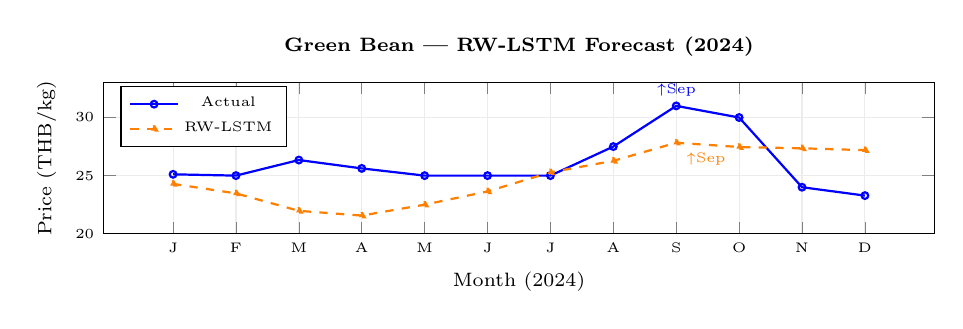
\begin{tikzpicture}
    \begin{axis}[
      width=\columnwidth, height=3.5cm,
      xlabel={\scriptsize Month (2024)}, ylabel={\scriptsize Price (THB/kg)},
      xticklabel style={font=\tiny}, yticklabel style={font=\tiny},
      xlabel style={font=\tiny}, ylabel style={font=\tiny},
      title={\scriptsize\bfseries Green Bean --- RW-LSTM Forecast (2024)},
      xtick={1,2,...,12},
      xticklabels={J,F,M,A,M,J,J,A,S,O,N,D},
      ymin=20, ymax=33, grid=major, grid style={gray!15},
      legend style={font=\tiny, at={(0.02,0.98)}, anchor=north west},
    ]
    \addplot[blue, thick, mark=o, mark size=1.2pt] coordinates {
      (1,25.11)(2,25.00)(3,26.34)(4,25.62)(5,25.00)(6,25.00)
      (7,25.00)(8,27.50)(9,31.00)(10,30.00)(11,24.00)(12,23.28)
    }; \addlegendentry{Actual}
    \addplot[orange, dashed, thick, mark=triangle*, mark size=1.2pt] coordinates {
      (1,24.29)(2,23.47)(3,21.97)(4,21.56)(5,22.50)(6,23.64)
      (7,25.28)(8,26.27)(9,27.83)(10,27.46)(11,27.35)(12,27.19)
    }; \addlegendentry{RW-LSTM}
    % Peak markers
    \node[font=\tiny, blue, above] at (axis cs:9,31.00) {$\uparrow$Sep};
    \node[font=\tiny, orange, below right] at (axis cs:9,27.83) {$\uparrow$Sep};
    \end{axis}
  \end{tikzpicture}
  \caption{Green bean 2024: RW-LSTM correctly predicts peak timing in Sep ($\Delta$Month~=~0) with the validated 5-year window, compared to Standard LSTM's 2-month error (Fig.~\ref{fig:lstm_gb_limit}).}
  \label{fig:rwlstm_gb}
\end{figure}

% --- Algorithm 1: RW-LSTM Training ---
\begin{algorithm}[htbp]
\SetAlgoLined
\KwIn{Price series $P$, window size $w$, target year $T$, sequence length $L{=}12$, prediction horizon $H{=}12$}
\KwOut{12-month forecast $\mathbf{F}$ for year $T$}
$\text{train\_data} \leftarrow P[\text{year} \in [T{-}w,\; T{-}1]]$\;
$\text{scaled} \leftarrow \text{MinMaxScaler.fit\_transform}(\text{train\_data})$\;
$\mathcal{S} \leftarrow \text{SeqDataset}(\text{scaled}, L, H)$ \tcp*{sliding windows}
Initialize 3-layer LSTM (hidden=32)\;
\For{epoch $= 1$ \KwTo $300$}{
  \ForEach{$(\mathbf{x}, \mathbf{y}) \in \text{DataLoader}(\mathcal{S})$}{
    $\ell \leftarrow \text{MSE}(\text{LSTM}(\mathbf{x}),\; \mathbf{y})$\;
    Backpropagate $\ell$; update parameters\;
  }
}
$\mathbf{F}_\text{scaled} \leftarrow \text{LSTM}(\text{scaled}[-L:])$\;
$\mathbf{F} \leftarrow \text{MinMaxScaler.inverse\_transform}(\mathbf{F}_\text{scaled})$\;
\Return{$\mathbf{F}$}
\caption{Rolling-Window LSTM Training and Prediction}
\label{alg:rwlstm}
\end{algorithm}

\subsubsection{Evaluation Metrics}

Model performance was evaluated using three metrics.

\textit{Mean Absolute Error (MAE):}
\begin{equation}
  \text{MAE} = \frac{1}{n}\sum_{t=1}^{n}|\hat{y}_t - y_t|
\end{equation}

\textit{Mean Absolute Percentage Error (MAPE):}
\begin{equation}
  \text{MAPE} = \frac{100\%}{n}\sum_{t=1}^{n}\left|\frac{\hat{y}_t - y_t}{y_t}\right|
\end{equation}

\textit{Forecast Accuracy\footnote{Defined as the complement of MAPE, not to be confused with classification accuracy.}:}
\begin{equation}
  \text{Forecast Accuracy} = 1 - \text{MAPE}
\end{equation}

Additionally, \textbf{Peak Timing Accuracy} was measured for the Rolling-Window LSTM, defined as the absolute difference in months between the predicted and actual peak price positions. This metric is critical because the scheduling system uses peak positions to determine harvest dates.

\subsection{Crop Planning Recommendation System}

\subsubsection{Problem Formulation}

The crop planning problem is formulated as a \textit{Weighted Job Scheduling Problem} (WJSP)~\cite{clrs2009, kleinberg2005}. Let $\mathcal{C} = \{c_1, c_2, \ldots, c_n\}$ be a set of $n$ candidate crops. Each crop $c_i$ is characterized by:
\begin{itemize}
  \item Growing duration $d_i$ (days),
  \item Yield $Y_i$ (kg/rai),
  \item Forecast price function $\hat{P}_i(t)$ over months $t \in \{1, \ldots, 12\}$,
  \item Peak harvest month $t_i^* = \arg\max_t \hat{P}_i(t) / \bar{P}_i$ (normalized),
  \item Planting start $s_i = t_i^* - d_i$, and
  \item Expected income $I_i = Y_i \times \hat{P}_i(t_i^*)$.
\end{itemize}

The objective is to find a non-overlapping schedule $S \subseteq \mathcal{C}$ that maximizes total income:
\begin{equation}
  \max_{S \subseteq \mathcal{C}} \sum_{c_i \in S} I_i \quad \text{s.t.} \quad [s_i, s_i + d_i) \cap [s_j, s_j + d_j) = \emptyset \;\; \forall\, c_i, c_j \in S,\; i \neq j
\end{equation}

This is a variant of the Weighted Interval Scheduling Problem, which is NP-hard in the general case with arbitrary job parameters~\cite{clrs2009}. For $n$ crops, an exhaustive search requires evaluating $O(n!)$ permutations (since placement order affects feasibility), while a dynamic programming approach can solve the weighted interval scheduling variant in $O(n \log n)$~\cite{kleinberg2005}. With $n = 4$ in this study, exhaustive enumeration ($4! = 24$ permutations) is trivial and serves as an exact benchmark.

\subsubsection{Phase 1: Job Definition from Forecasts}

Rolling-Window LSTM forecasts are normalized by dividing each crop's price series by its mean, enabling cross-crop comparison. The peak normalized price date~(argmax) defines the harvest date---the optimal selling time. The planting date is then computed by subtracting the growing period:
\begin{equation}
  t_{\text{plant}} = t_{\text{harvest}} - d_{\text{grow}}
\end{equation}

Table~\ref{tab:agro} lists the agronomic constants used.

\begin{table}[htbp]
  \centering
  \caption{Agronomic Constants per Crop}
  \label{tab:agro}
  \begin{tabular}{lcc}
    \toprule
    \textbf{Crop} & \textbf{Growing Days} & \textbf{Yield (kg/rai)} \\
    \midrule
    Cassava & 250 & 3,500 \\
    Corn & 120 & 1,500 \\
    Green Bean & 80 & 245 \\
    Soybean & 90 & 300 \\
    \bottomrule
  \end{tabular}
\end{table}

Each crop's expected income is computed as:
\begin{equation}
  I_i = Y_i \times P_i^{\text{peak}} \times A
  \label{eq:income}
\end{equation}
where $Y_i$ is yield (kg/rai), $P_i^{\text{peak}}$ is the price at peak (THB/kg), and $A$ is area. In this study, $A = 1$~rai for all computations. Yield values are national agronomic averages from OAE data and are treated as deterministic constants. This simplification is discussed in Section~\ref{sec:sensitivity}.

\subsubsection{Phase 2: Greedy Scheduling}

Since independently optimal positions for each crop may overlap, a scheduling algorithm is required. Fig.~\ref{fig:flowchart} presents the greedy scheduling process as a flowchart.

% --- Fig. 8: Greedy Scheduling Flowchart ---
\begin{figure*}[htbp]
  \centering
  \resizebox{\textwidth}{!}{%
  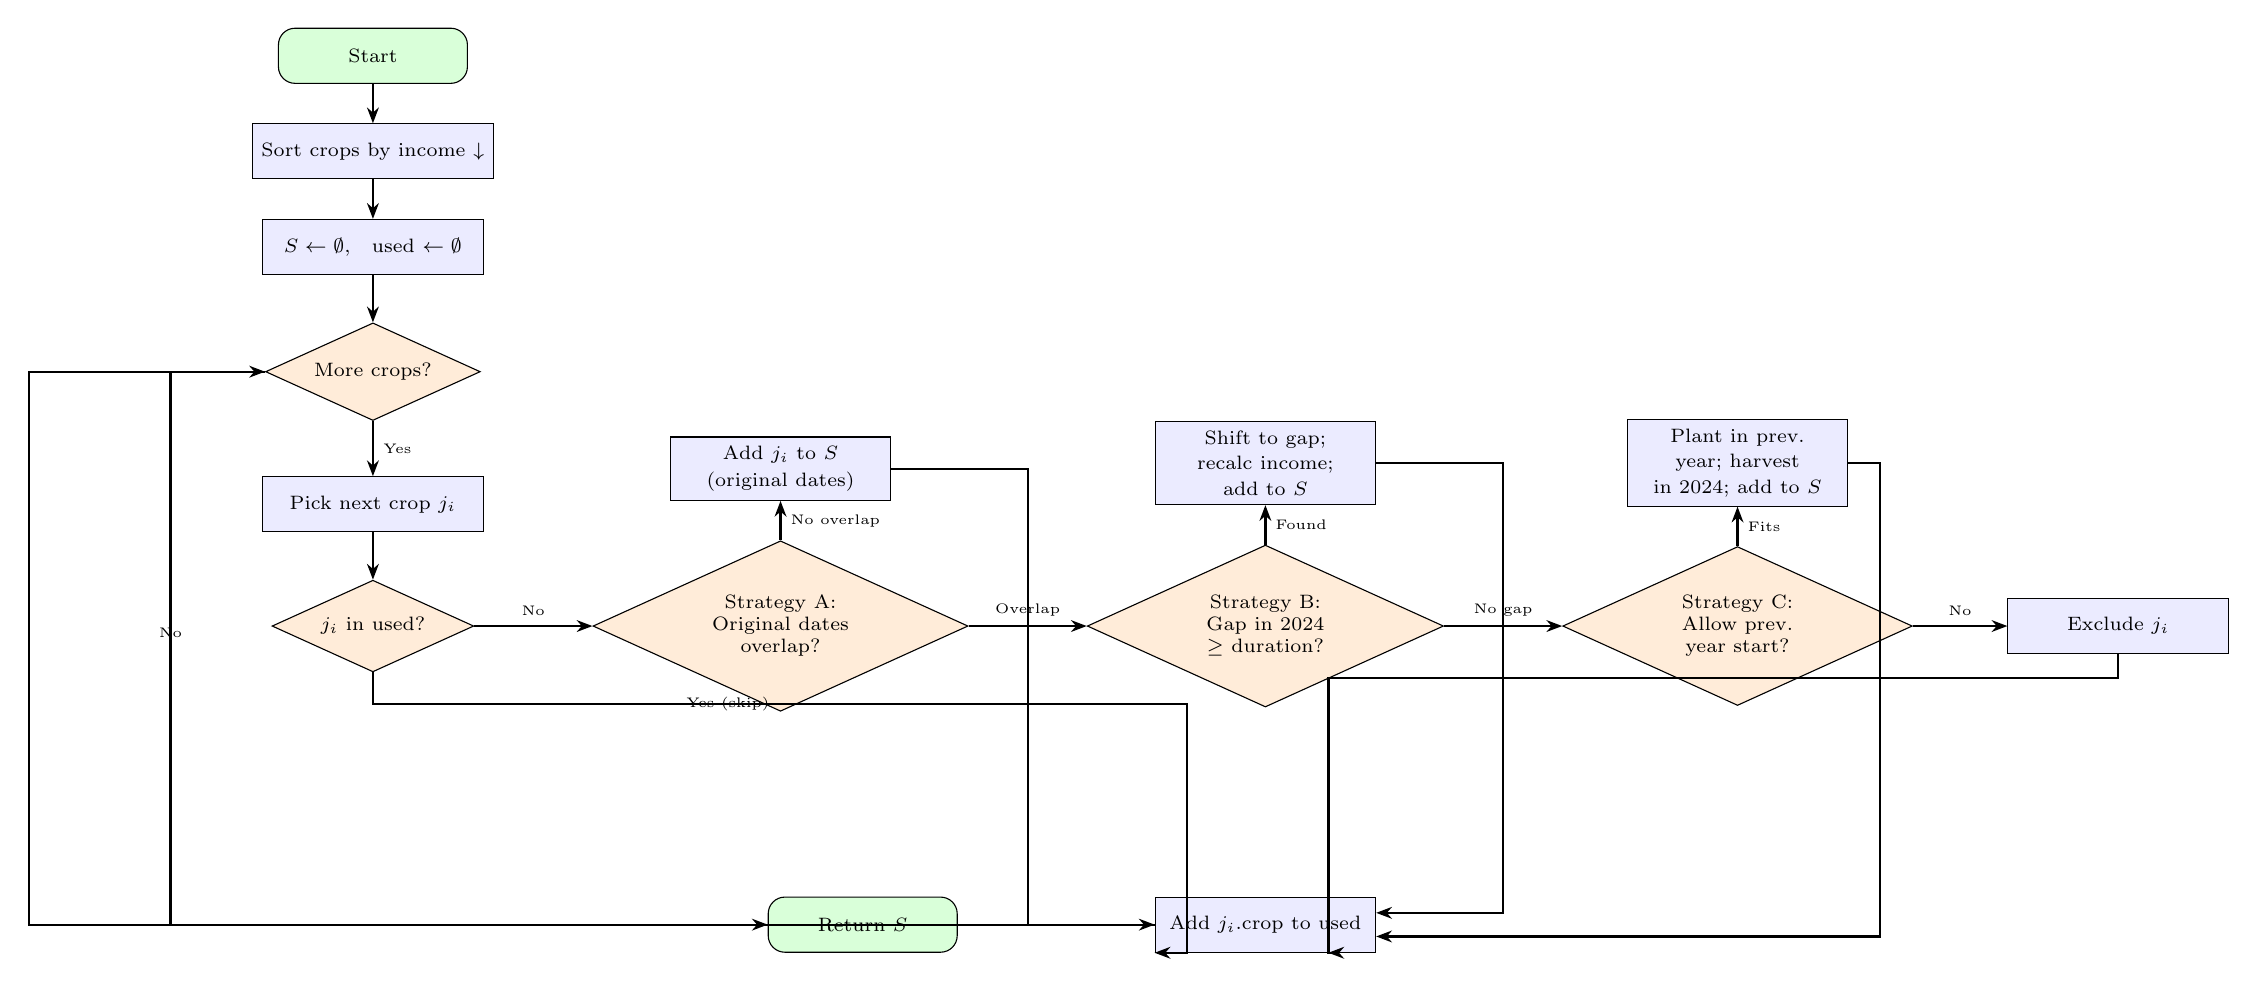
\begin{tikzpicture}[node distance=0.5cm and 0.6cm]
    % Start
    \node[startstop] (start) {Start};

    % Sort
    \node[process, below=0.5cm of start] (sort) {Sort crops by income $\downarrow$};

    % Init
    \node[process, below=of sort] (init) {$S \leftarrow \emptyset$, \; used $\leftarrow \emptyset$};

    % Loop
    \node[decision, below=0.6cm of init] (hasnext) {More crops?};

    % Pick next
    \node[process, below=0.7cm of hasnext] (pick) {Pick next crop $j_i$};

    % Used check
    \node[decision, below=0.6cm of pick] (usedcheck) {$j_i$ in used?};

    % Strategy A
    \node[decision, right=1.5cm of usedcheck] (stratA) {
      \begin{tabular}{c}
        Strategy A:\\Original dates\\overlap?
      \end{tabular}
    };

    % A success
    \node[process, above=0.5cm of stratA] (addA) {\shortstack{Add $j_i$ to $S$\\(original dates)}};

    % Strategy B
    \node[decision, right=1.5cm of stratA] (stratB) {
      \begin{tabular}{c}
        Strategy B:\\Gap in 2024\\$\geq$ duration?
      \end{tabular}
    };

    % B success
    \node[process, above=0.5cm of stratB] (addB) {\shortstack{Shift to gap;\\recalc income;\\add to $S$}};

    % Strategy C
    \node[decision, right=1.5cm of stratB] (stratC) {
      \begin{tabular}{c}
        Strategy C:\\Allow prev.\\year start?
      \end{tabular}
    };

    % C success
    \node[process, above=0.5cm of stratC] (addC) {\shortstack{Plant in prev.\\year; harvest\\in 2024; add to $S$}};

    % Exclude
    \node[process, right=1.2cm of stratC] (exclude) {Exclude $j_i$};

    % Mark used
    \node[process, below=2.4cm of stratB] (markused) {Add $j_i$.crop to used};

    % End
    \node[startstop, left=2.5cm of markused] (end) {Return $S$};

% === Arrows ===
    \draw[arrow] (start) -- (sort);
    \draw[arrow] (sort) -- (init);
    \draw[arrow] (init) -- (hasnext);
    % Has next
    \draw[arrow] (hasnext) -- node[right, font=\tiny] {Yes} (pick);
    \draw[arrow] (hasnext.west) -- ++(-1.2,0) |- node[near start, above, font=\tiny] {No} (end);
    % Used check
    \draw[arrow] (pick) -- (usedcheck);
    \draw[arrow] (usedcheck) -- node[above, font=\tiny] {No} (stratA);

    % Used check Yes: go down then right into markused from the left side
    \draw[arrow] (usedcheck.south) -- ++(0,-0.4)
      -| node[near start, left, font=\tiny] {Yes (skip)} ([xshift=-1cm]markused.south) -- (markused.south west);

    % Strategy A
    \draw[arrow] (stratA) -- node[right, font=\tiny] {No overlap} (addA);
    \draw[arrow] (stratA) -- node[above, font=\tiny] {Overlap} (stratB);

    % Strategy B
    \draw[arrow] (stratB) -- node[right, font=\tiny] {Found} (addB);
    \draw[arrow] (stratB) -- node[above, font=\tiny] {No gap} (stratC);

    % Strategy C
    \draw[arrow] (stratC) -- node[right, font=\tiny] {Fits} (addC);
    \draw[arrow] (stratC) -- node[above, font=\tiny] {No} (exclude);

    % --- Success paths into markused ---
    % Route via gaps BETWEEN the diamonds to avoid crossing nodes.

    % addA -> markused: via gap between stratA and stratB
    \draw[arrow] (addA.east) -| ($(stratA.east)!0.5!(stratB.west)$) |- (markused);

    % addB -> markused: via gap between stratB and stratC
    \draw[arrow] (addB.east) -| ($(stratB.east)!0.5!(stratC.west)$) |- ([yshift=0.15cm]markused.east);

    % addC -> markused: route right from addC then down
    \draw[arrow] (addC.east) -- ++(0.4,0) |- ([yshift=-0.15cm]markused.east);

    % Exclude -> markused: go down then into markused from the south
    \draw[arrow] (exclude.south) -- ++(0,-0.3) -| ([xshift=0.8cm]markused.south) -- (markused);

    % Loop back
    \draw[arrow] (markused.west) -| ([xshift=-3cm]hasnext.west) -- (hasnext.west);
  \end{tikzpicture}}%
  \caption{Flowchart of the Greedy Crop Scheduling algorithm. Crops are processed in descending income order. For each crop, three placement strategies are attempted sequentially: (A)~original peak-optimal dates, (B)~shifted to an available gap within the target year, (C)~planting in the previous year with harvest in the target year. If none succeeds, the crop is excluded.}
  \label{fig:flowchart}
\end{figure*}

Algorithm~\ref{alg:greedy} formalizes the flowchart as pseudocode.

% --- Algorithm 2: Greedy Scheduling ---
\begin{algorithm}[htbp]
\SetAlgoLined
\KwIn{Crop candidates $\mathcal{C}$ with income $I_i$, duration $d_i$, harvest date $t_i^*$}
\KwOut{Non-overlapping schedule $S$}
Sort $\mathcal{C}$ by $I_i$ in descending order\;
$S \leftarrow \emptyset$;\; $\text{used} \leftarrow \emptyset$;\; $\text{intervals} \leftarrow \emptyset$\;
\ForEach{candidate $c_i \in \mathcal{C}$}{
  \If{$c_i.\text{crop} \in \text{used}$}{\textbf{continue}\;}
  $s_i \leftarrow t_i^* - d_i$\;
  \tcp{Strategy A: original dates}
  \If{$[s_i, t_i^*)$ does not overlap any interval in $\text{intervals}$}{
    $S \leftarrow S \cup \{c_i\}$ with original dates\;
  }
  \tcp{Strategy B: shift to available gap}
  \ElseIf{$\exists$ gap $[g_s, g_e)$ in $\text{intervals}$ where $g_e - g_s \geq d_i$}{
    Shift $c_i$ to gap; recalculate $I_i$ at new harvest date\;
    $S \leftarrow S \cup \{c_i\}$ with shifted dates\;
  }
  \tcp{Strategy C: plant in previous year}
  \ElseIf{$c_i$ can start in previous year with harvest in target year}{
    $S \leftarrow S \cup \{c_i\}$ with adjusted dates\;
  }
  \Else{Exclude $c_i$\;}
  $\text{used} \leftarrow \text{used} \cup \{c_i.\text{crop}\}$\;
  Update $\text{intervals}$\;
}
\Return{$S$}
\caption{Greedy Crop Scheduling}
\label{alg:greedy}
\end{algorithm}

The algorithm enforces four constraints: (1)~non-overlap---one crop per plot at any time; (2)~one planting per crop; (3)~harvest must fall within the target year; (4)~fixed area of 1~rai.

\textit{Complexity analysis.} Sorting requires $O(n \log n)$. For each of the $n$ crops, gap-finding checks against at most $|S|$ intervals, yielding $O(n^2)$ worst-case overall. For our $n = 4$ crops, this is negligible. Exhaustive enumeration requires $O(n!)$, which is trivial for $n = 4$ ($4! = 24$) but infeasible for larger crop sets ($15! \approx 1.3 \times 10^{12}$). Dynamic programming for weighted interval scheduling achieves $O(n \log n)$~\cite{kleinberg2005} and is recommended for $n > 10$.

\textit{Numerical example (Strategy~B).} Consider corn, which the greedy algorithm schedules second. Its optimal harvest date is February (peak price 13.58~THB/kg), but this overlaps with the first-scheduled crop. Strategy~B identifies a gap starting after the first crop's harvest and shifts corn to harvest in June, yielding a lower price of 12.71~THB/kg. The income drops from $1{,}500 \times 13.58 = 20{,}370$~THB to $1{,}500 \times 12.71 = 19{,}065$~THB---a 6.4\% reduction accepted as the cost of non-overlap.

As a greedy heuristic, the algorithm does not guarantee global optimality---scheduling a high-income crop first may block two medium-income crops with higher combined revenue. To verify solution quality, we additionally perform an exhaustive search over all $4! = 24$ permutations. The greedy heuristic is presented as the general-purpose algorithm applicable to larger crop sets where exhaustive search becomes infeasible.

\subsection{Web Application}

% --- Fig. 9: Web Application Architecture ---
\begin{figure}[htbp]
  \centering
  \resizebox{\columnwidth}{!}{%
  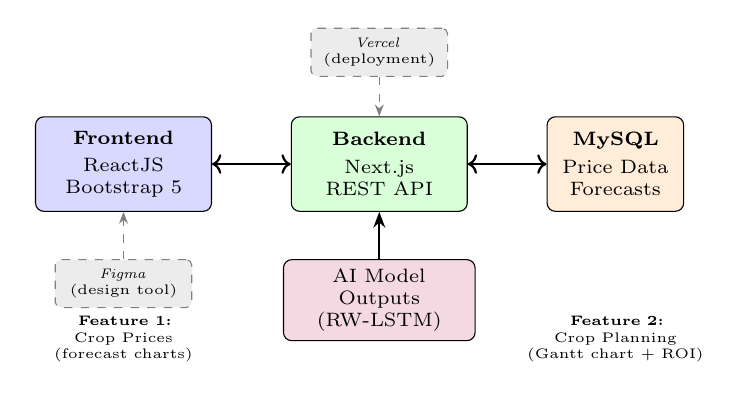
\begin{tikzpicture}[node distance=0.5cm and 0.8cm]
    % Frontend
    \node[block=blue!15, text width=2cm, align=center, minimum height=1.2cm] (fe) {
      \textbf{Frontend}\\[2pt]
      ReactJS\\
      Bootstrap 5
    };

    % Backend
    \node[block=green!15, right=1cm of fe, text width=2cm, align=center, minimum height=1.2cm] (be) {
      \textbf{Backend}\\[2pt]
      Next.js\\
      REST API
    };

    % Database
    \node[block=orange!15, right=1cm of be, text width=1.5cm, align=center, minimum height=1.2cm] (db) {
      \textbf{MySQL}\\[2pt]
      Price Data\\
      Forecasts
    };

    % AI Models
    \node[block=purple!15, below=0.6cm of be, text width=2.2cm, align=center] (ai) {AI Model Outputs\\(RW-LSTM)};

    % Development tools (not runtime)
    \node[smallblock=gray!15, below=0.6cm of fe, text width=1.5cm, align=center, draw=gray, dashed] (figma) {\textit{Figma}\\{\tiny (design tool)}};

    % Deployment
    \node[smallblock=gray!15, above=0.5cm of be, text width=1.5cm, align=center, draw=gray, dashed] (vercel) {\textit{Vercel}\\{\tiny (deployment)}};

    % Arrows
    \draw[arrow, <->] (fe) -- (be);
    \draw[arrow, <->] (be) -- (db);
    \draw[arrow] (ai) -- (be);
    \draw[-{Stealth[length=1.5mm]}, gray, dashed, thin] (figma) -- (fe);
    \draw[-{Stealth[length=1.5mm]}, gray, dashed, thin] (vercel) -- (be);

    % Features
    \node[below=1.2cm of fe, font=\tiny, text width=2.2cm, align=center] (f1) {\textbf{Feature 1:} Crop Prices\\(forecast charts)};
    \node[below=1.2cm of db, font=\tiny, text width=2.2cm, align=center] (f2) {\textbf{Feature 2:} Crop Planning\\(Gantt chart + ROI)};
  \end{tikzpicture}}%
  \caption{Web application architecture. The frontend communicates with a Next.js backend connected to MySQL for data storage. AI model outputs feed into the backend for real-time recommendations.}
  \label{fig:webapp}
\end{figure}

The CropPlanner web application was built with ReactJS and Bootstrap~5 for the frontend, Next.js with MySQL for the backend, prototyped in Figma, and deployed on Vercel. The backend exposes two REST~API endpoints: \texttt{/api/forecast?crop=\{name\}} returns 12-month RW-LSTM price predictions as JSON, and \texttt{/api/schedule?start=\{month\}\&area=\{rai\}} returns the optimized Gantt chart data with a financial summary.

The application provides two main features: (1)~\textbf{Crop Prices}---displaying AI-predicted price charts for all four crops; and (2)~\textbf{Crop Planning}---accepting start month and area inputs, then presenting a Gantt chart recommendation with financial summaries (income, expenses, profit, and ROI).

\textit{UX Design Rationale.} The interface was designed with simplicity as the primary concern, targeting non-technical users in rural areas. Line charts were chosen for price forecasts because they are the most widely understood format for temporal data; Gantt charts were chosen for scheduling because they directly represent time slots on a calendar---a mental model familiar to farmers who think in planting seasons. Each crop is assigned a consistent color across all views (cassava: brown, corn: gold, green bean: green, soybean: blue) to reduce cognitive load. The responsive layout ensures usability on both desktop and mobile devices.

\textit{Database Schema.} The MySQL backend stores three core tables: \texttt{crops} (crop name, growing days, yield per rai), \texttt{forecasts} (crop ID, month, predicted price, model name), and \texttt{schedules} (session ID, crop ID, start date, end date, strategy, projected income). Pre-computed RW-LSTM forecasts are loaded into the \texttt{forecasts} table at deployment; the scheduling algorithm runs on-demand when users submit a planning request.

\textit{API Design.} The forecast endpoint returns a JSON array of monthly predictions:

\begin{verbatim}
GET /api/forecast?crop=cassava
[{"month":"2024-01","price":2.57},
 {"month":"2024-02","price":2.50}, ...]
\end{verbatim}

\noindent The schedule endpoint accepts start month and area, runs Algorithm~\ref{alg:greedy}, and returns the resulting Gantt entries with per-crop income breakdowns. This separation of concerns allows the forecast models to be updated independently of the scheduling logic.

The application was deployed on Vercel with the Next.js backend serving these REST~API endpoints. The interface is responsive across desktop and mobile devices, ensuring accessibility for farmers in rural areas with limited computing resources.

% ============================================================
% V. RESULTS
% ============================================================
\section{Results}
\label{sec:results}

\subsection{Model Comparison}

Tables~\ref{tab:mape} and~\ref{tab:accuracy} present MAPE and Accuracy results for the 2024 test year. Bold values indicate the best result per crop.

\begin{table}[htbp]
  \centering
  \caption{MAPE (\%) for 2024 Test Year}
  \label{tab:mape}
  \begin{tabular}{lcccc}
    \toprule
    \textbf{Crop} & \textbf{LSTM} & \textbf{Trans.} & \textbf{ARIMA} & \textbf{RW-LSTM} \\
    \midrule
    Cassava    & \textbf{4.81}  & 9.32  & 24.71 & 23.18 \\
    Corn       & \textbf{6.43}  & 15.09 & 8.10  & 13.32 \\
    Green Bean & 7.20           & 6.34  & \textbf{6.08}  & 9.36  \\
    Soybean    & 9.44           & \textbf{5.71} & 6.99 & 22.38 \\
    \midrule
    \textbf{Average} & \textbf{7.07} & 9.12 & 11.47 & 17.06 \\
    \bottomrule
  \end{tabular}
\end{table}

\begin{table}[htbp]
  \centering
  \caption{Forecast Accuracy (\%) for 2024 Test Year}
  \label{tab:accuracy}
  \begin{tabular}{lcccc}
    \toprule
    \textbf{Crop} & \textbf{LSTM} & \textbf{Trans.} & \textbf{ARIMA} & \textbf{RW-LSTM} \\
    \midrule
    Cassava    & \textbf{95.33} & 89.99 & 77.74 & 75.80 \\
    Corn       & \textbf{93.29} & 84.29 & 92.03 & 87.02 \\
    Green Bean & 92.51          & \textbf{93.50} & 93.45 & 90.69 \\
    Soybean    & 90.57          & \textbf{94.18} & 92.82 & 77.90 \\
    \midrule
    \textbf{Average} & \textbf{92.93} & 90.49 & 89.01 & 82.85 \\
    \bottomrule
  \end{tabular}
\end{table}

No single model dominates across all crops. Standard LSTM achieves the highest average forecast accuracy (92.93\%) and performs best for cassava and corn. Transformer excels for green bean (93.50\%) and soybean (94.18\%). ARIMA performs notably poorly for cassava (77.74\%) due to structural breaks violating stationarity assumptions. Rolling-Window LSTM, with window sizes selected via validation rather than test-set feedback, achieves a lower average accuracy (82.85\%) than the other models. This demonstrates the effect of proper hyperparameter selection: the original window sizes, which were tuned using test-year feedback, produced artificially inflated accuracy figures.

Fig.~\ref{fig:boxplot} shows the distribution of monthly absolute percentage errors across all 48~predictions (4~crops~$\times$~12~months) per model. While LSTM and ARIMA have similar median errors ($\sim$6--7\%), ARIMA exhibits far higher variance and three outliers exceeding 40\% (all from cassava Q4, where ARIMA's stationarity assumption fails most severely). Transformer shows moderate variance with a maximum of 28\%, concentrated in corn's mid-year spike. RW-LSTM has the highest median error (16.2\%) and widest interquartile range, reflecting its trade-off of pointwise accuracy for peak timing. The narrow IQR of LSTM (3.5--10.0\%) indicates the most consistent predictions across crops and months.

% --- Fig: Error Distribution Box Plot ---
\begin{figure}[htbp]
  \centering
  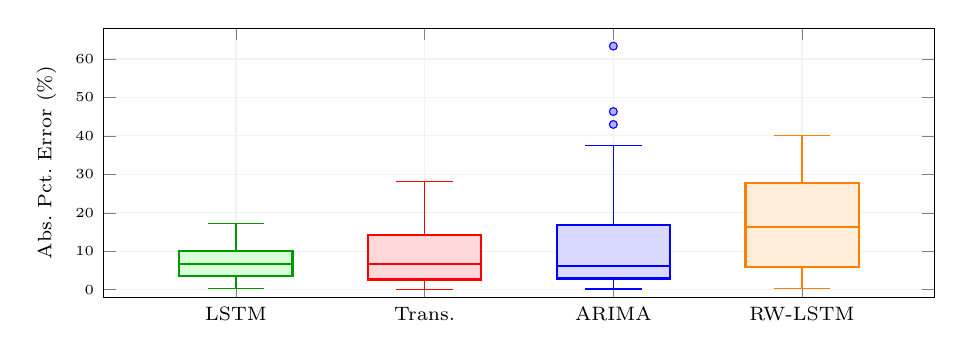
\begin{tikzpicture}
    \begin{axis}[
      width=\columnwidth, height=5cm,
      ylabel={\scriptsize Abs.\ Pct.\ Error (\%)},
      ylabel style={font=\scriptsize},
      xticklabel style={font=\scriptsize},
      yticklabel style={font=\tiny},
      xtick={1,2,3,4},
      xticklabels={LSTM, Trans., ARIMA, RW-LSTM},
      xmin=0.3, xmax=4.7,
      ymin=-2, ymax=68,
      grid=major, grid style={gray!10},
      ytick={0,10,20,30,40,50,60},
    ]
    % LSTM: min=0.28, Q1=3.50, med=6.68, Q3=9.97, max=17.29
    \draw[thick, green!60!black, fill=green!15] (axis cs:0.7,3.50) rectangle (axis cs:1.3,9.97);
    \draw[thick, green!60!black] (axis cs:0.7,6.68) -- (axis cs:1.3,6.68); % median
    \draw[green!60!black] (axis cs:1,0.28) -- (axis cs:1,3.50); % lower whisker
    \draw[green!60!black] (axis cs:1,9.97) -- (axis cs:1,17.29); % upper whisker
    \draw[green!60!black] (axis cs:0.85,0.28) -- (axis cs:1.15,0.28); % lower cap
    \draw[green!60!black] (axis cs:0.85,17.29) -- (axis cs:1.15,17.29); % upper cap

    % Transformer: min=0.10, Q1=2.63, med=6.78, Q3=14.32, max=28.19
    \draw[thick, red, fill=red!15] (axis cs:1.7,2.63) rectangle (axis cs:2.3,14.32);
    \draw[thick, red] (axis cs:1.7,6.78) -- (axis cs:2.3,6.78);
    \draw[red] (axis cs:2,0.10) -- (axis cs:2,2.63);
    \draw[red] (axis cs:2,14.32) -- (axis cs:2,28.19);
    \draw[red] (axis cs:1.85,0.10) -- (axis cs:2.15,0.10);
    \draw[red] (axis cs:1.85,28.19) -- (axis cs:2.15,28.19);

    % ARIMA: min=0.18, Q1=2.93, med=6.13, Q3=16.77, whisker_hi=37.53, outliers 42.98, 46.33, 63.35
    \draw[thick, blue, fill=blue!15] (axis cs:2.7,2.93) rectangle (axis cs:3.3,16.77);
    \draw[thick, blue] (axis cs:2.7,6.13) -- (axis cs:3.3,6.13);
    \draw[blue] (axis cs:3,0.18) -- (axis cs:3,2.93);
    \draw[blue] (axis cs:3,16.77) -- (axis cs:3,37.53);
    \draw[blue] (axis cs:2.85,0.18) -- (axis cs:3.15,0.18);
    \draw[blue] (axis cs:2.85,37.53) -- (axis cs:3.15,37.53);
    % Outliers
    \node[circle, draw=blue, fill=blue!30, inner sep=1pt, font=\tiny] at (axis cs:3,42.98) {};
    \node[circle, draw=blue, fill=blue!30, inner sep=1pt, font=\tiny] at (axis cs:3,46.33) {};
    \node[circle, draw=blue, fill=blue!30, inner sep=1pt, font=\tiny] at (axis cs:3,63.35) {};

    % RW-LSTM: min=0.20, Q1=5.95, med=16.22, Q3=27.70, max=40.18
    \draw[thick, orange, fill=orange!15] (axis cs:3.7,5.95) rectangle (axis cs:4.3,27.70);
    \draw[thick, orange] (axis cs:3.7,16.22) -- (axis cs:4.3,16.22);
    \draw[orange] (axis cs:4,0.20) -- (axis cs:4,5.95);
    \draw[orange] (axis cs:4,27.70) -- (axis cs:4,40.18);
    \draw[orange] (axis cs:3.85,0.20) -- (axis cs:4.15,0.20);
    \draw[orange] (axis cs:3.85,40.18) -- (axis cs:4.15,40.18);
    \end{axis}
  \end{tikzpicture}
  \caption{Distribution of monthly absolute percentage errors across all 48~predictions (4~crops~$\times$~12~months) per model. LSTM has the tightest distribution; ARIMA has three outliers exceeding 40\% (cassava Q4); RW-LSTM trades higher median error for better peak timing.}
  \label{fig:boxplot}
\end{figure}

% Individual RW-LSTM plots removed; all four crops shown in Fig.~\ref{fig:rwlstm_all}.

\subsubsection{Peak Timing Accuracy}

While Rolling-Window LSTM has a higher average MAPE than Standard LSTM with proper validation-based window selection, its key advantage is peak timing accuracy (Table~\ref{tab:peak}).

\begin{table}[htbp]
  \centering
  \caption{Peak Timing Accuracy --- Rolling-Window LSTM}
  \label{tab:peak}
  \begin{tabular}{lccccc}
    \toprule
    \textbf{Crop} & \textbf{Actual} & \textbf{Pred.} & $\boldsymbol{\Delta}$\textbf{Mo.} & $\boldsymbol{\Delta}$\textbf{Price} & \textbf{Rating} \\
    \midrule
    Cassava    & Jan & Jan & 0 & 29.57\% & Excellent \\
    Corn       & Jul & Feb & 5 & 9.12\%  & Poor \\
    Green Bean & Sep & Sep & 0 & 10.24\% & Excellent \\
    Soybean    & Apr & Mar & 1 & 20.44\% & Excellent \\
    \bottomrule
  \end{tabular}
\end{table}

Two of four crops (cassava and green bean) have exact peak month predictions, and soybean is within one month (Fig.~\ref{fig:rwlstm_all}). Corn's peak prediction is five months off, reflecting the difficulty of capturing its mid-year price spike with a short (6-year) window. Note that the $\Delta$Price column reflects overall forecast error at the peak month, not scheduling quality: the scheduling system uses only the peak month position to set the harvest date, while income is computed from the predicted price at that month. Cassava's high $\Delta$Price (29.57\%) despite exact peak timing indicates the forecast underestimates the price level but correctly identifies \textit{when} to harvest. Despite lower overall MAPE compared to the test-tuned configuration, the validated model retains strong peak timing for three of four crops---critical for the scheduling system.

\subsubsection{Cross-Model Analysis and Ensemble Potential}

The per-model comparison figures (Fig.~\ref{fig:cross_model}) reveal distinct model behaviors across crops. LSTM and Transformer tend to produce smooth forecasts that track the general price level well but miss sharp peaks; ARIMA captures seasonal periodicity but diverges when stationarity is violated; RW-LSTM sacrifices price-level accuracy for better peak timing.

% --- Fig: Cross-Model Comparison Grid (TikZ) ---
\begin{figure*}[htbp]
  \centering
  \resizebox{\textwidth}{!}{%
  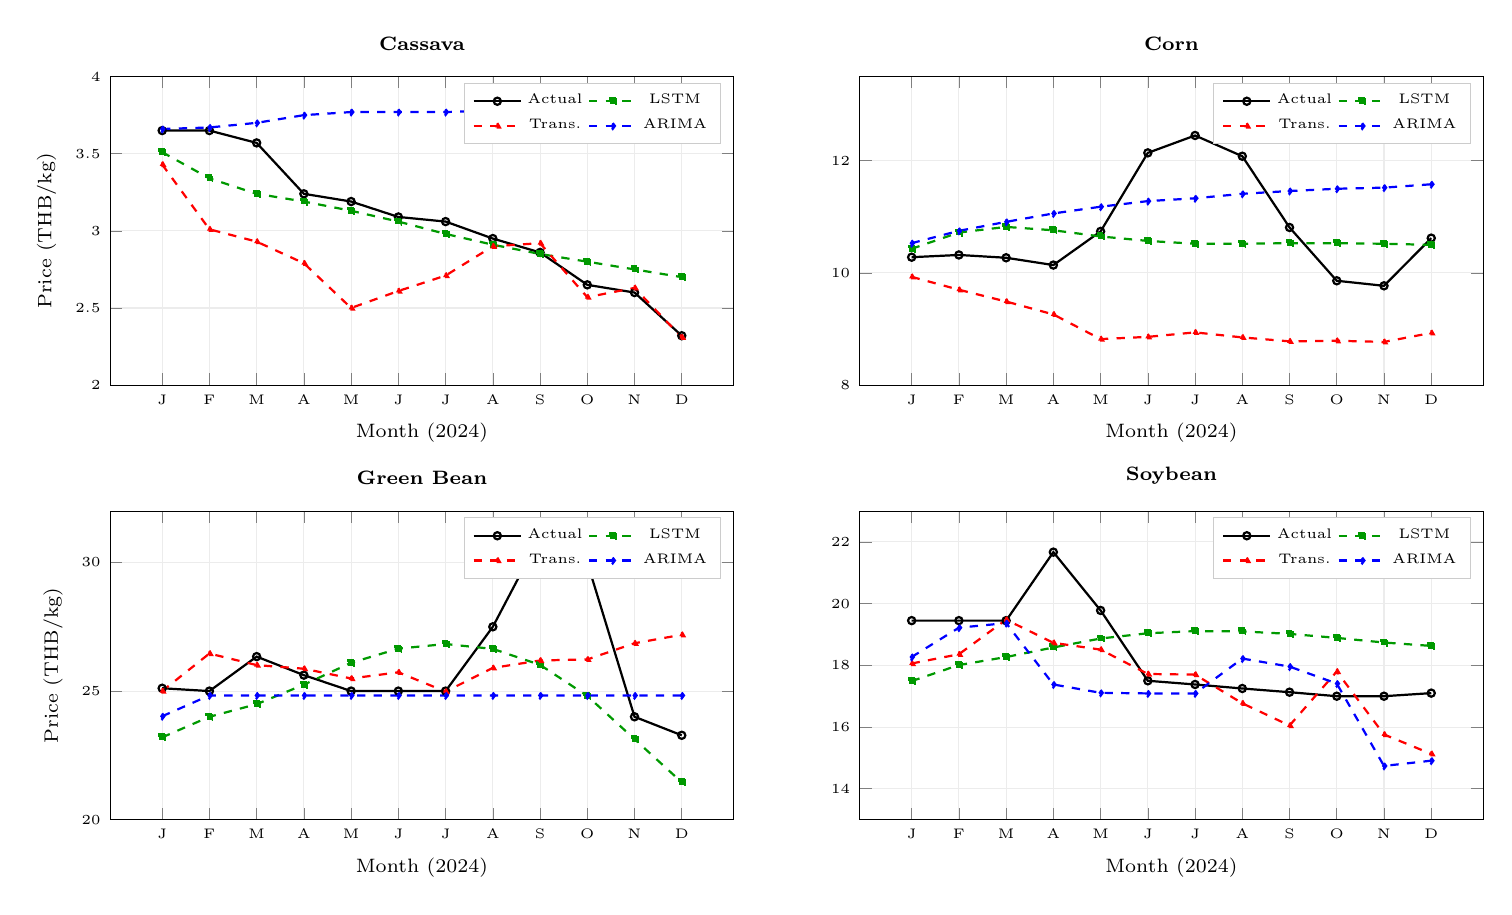
\begin{tikzpicture}
    \begin{groupplot}[
      group style={group size=2 by 2, horizontal sep=1.6cm, vertical sep=1.6cm},
      width=9.5cm, height=5.5cm,
      xlabel={\scriptsize Month (2024)},
      xlabel style={font=\scriptsize},
      ylabel style={font=\scriptsize},
      xticklabel style={font=\tiny},
      yticklabel style={font=\tiny},
      title style={font=\scriptsize\bfseries},
      grid=major, grid style={gray!15},
      xtick={1,2,...,12},
      xticklabels={J,F,M,A,M,J,J,A,S,O,N,D},
      legend style={font=\tiny, at={(0.98,0.98)}, anchor=north east, legend columns=2, draw=gray!40},
      every axis plot/.append style={thick, mark size=1.3pt},
    ]

    % === Cassava ===
    \nextgroupplot[title={Cassava}, ylabel={\scriptsize Price (THB/kg)}, ymin=2.0, ymax=4.0]
    \addplot[black, mark=o] coordinates {
      (1,3.65)(2,3.65)(3,3.57)(4,3.24)(5,3.19)(6,3.09)
      (7,3.06)(8,2.95)(9,2.86)(10,2.65)(11,2.60)(12,2.32)
    }; \addlegendentry{Actual}
    \addplot[green!60!black, dashed, mark=square*, mark options={fill=green!60!black, scale=0.8}] coordinates {
      (1,3.51)(2,3.34)(3,3.24)(4,3.19)(5,3.13)(6,3.06)
      (7,2.98)(8,2.91)(9,2.85)(10,2.80)(11,2.75)(12,2.70)
    }; \addlegendentry{LSTM}
    \addplot[red, dashed, mark=triangle*, mark options={fill=red, scale=0.8}] coordinates {
      (1,3.43)(2,3.01)(3,2.93)(4,2.79)(5,2.50)(6,2.61)
      (7,2.71)(8,2.90)(9,2.92)(10,2.57)(11,2.63)(12,2.31)
    }; \addlegendentry{Trans.}
    \addplot[blue, dashed, mark=diamond*, mark options={fill=blue, scale=0.8}] coordinates {
      (1,3.66)(2,3.67)(3,3.70)(4,3.75)(5,3.77)(6,3.77)
      (7,3.77)(8,3.78)(9,3.79)(10,3.79)(11,3.80)(12,3.79)
    }; \addlegendentry{ARIMA}

    % === Corn ===
    \nextgroupplot[title={Corn}, ymin=8.0, ymax=13.5]
    \addplot[black, mark=o] coordinates {
      (1,10.28)(2,10.32)(3,10.27)(4,10.14)(5,10.74)(6,12.14)
      (7,12.45)(8,12.08)(9,10.81)(10,9.86)(11,9.77)(12,10.62)
    }; \addlegendentry{Actual}
    \addplot[green!60!black, dashed, mark=square*, mark options={fill=green!60!black, scale=0.8}] coordinates {
      (1,10.43)(2,10.72)(3,10.82)(4,10.76)(5,10.65)(6,10.57)
      (7,10.52)(8,10.52)(9,10.53)(10,10.53)(11,10.52)(12,10.50)
    }; \addlegendentry{LSTM}
    \addplot[red, dashed, mark=triangle*, mark options={fill=red, scale=0.8}] coordinates {
      (1,9.93)(2,9.70)(3,9.49)(4,9.26)(5,8.82)(6,8.86)
      (7,8.94)(8,8.85)(9,8.78)(10,8.79)(11,8.77)(12,8.93)
    }; \addlegendentry{Trans.}
    \addplot[blue, dashed, mark=diamond*, mark options={fill=blue, scale=0.8}] coordinates {
      (1,10.53)(2,10.75)(3,10.91)(4,11.06)(5,11.18)(6,11.28)
      (7,11.33)(8,11.41)(9,11.46)(10,11.50)(11,11.52)(12,11.58)
    }; \addlegendentry{ARIMA}

    % === Green Bean ===
    \nextgroupplot[title={Green Bean}, ylabel={\scriptsize Price (THB/kg)}, ymin=20, ymax=32]
    \addplot[black, mark=o] coordinates {
      (1,25.11)(2,25.00)(3,26.34)(4,25.62)(5,25.00)(6,25.00)
      (7,25.00)(8,27.50)(9,31.00)(10,30.00)(11,24.00)(12,23.28)
    }; \addlegendentry{Actual}
    \addplot[green!60!black, dashed, mark=square*, mark options={fill=green!60!black, scale=0.8}] coordinates {
      (1,23.20)(2,24.00)(3,24.49)(4,25.25)(5,26.10)(6,26.65)
      (7,26.83)(8,26.64)(9,26.02)(10,24.81)(11,23.13)(12,21.45)
    }; \addlegendentry{LSTM}
    \addplot[red, dashed, mark=triangle*, mark options={fill=red, scale=0.8}] coordinates {
      (1,25.00)(2,26.46)(3,26.01)(4,25.87)(5,25.49)(6,25.73)
      (7,24.98)(8,25.90)(9,26.19)(10,26.23)(11,26.86)(12,27.19)
    }; \addlegendentry{Trans.}
    \addplot[blue, dashed, mark=diamond*, mark options={fill=blue, scale=0.8}] coordinates {
      (1,24.02)(2,24.83)(3,24.83)(4,24.83)(5,24.83)(6,24.83)
      (7,24.83)(8,24.83)(9,24.83)(10,24.83)(11,24.83)(12,24.83)
    }; \addlegendentry{ARIMA}

    % === Soybean ===
    \nextgroupplot[title={Soybean}, ymin=13, ymax=23]
    \addplot[black, mark=o] coordinates {
      (1,19.45)(2,19.45)(3,19.45)(4,21.67)(5,19.78)(6,17.50)
      (7,17.38)(8,17.25)(9,17.13)(10,17.00)(11,17.00)(12,17.10)
    }; \addlegendentry{Actual}
    \addplot[green!60!black, dashed, mark=square*, mark options={fill=green!60!black, scale=0.8}] coordinates {
      (1,17.49)(2,18.01)(3,18.27)(4,18.58)(5,18.87)(6,19.04)
      (7,19.11)(8,19.10)(9,19.02)(10,18.89)(11,18.74)(12,18.63)
    }; \addlegendentry{LSTM}
    \addplot[red, dashed, mark=triangle*, mark options={fill=red, scale=0.8}] coordinates {
      (1,18.06)(2,18.36)(3,19.48)(4,18.73)(5,18.51)(6,17.72)
      (7,17.70)(8,16.77)(9,16.05)(10,17.80)(11,15.76)(12,15.13)
    }; \addlegendentry{Trans.}
    \addplot[blue, dashed, mark=diamond*, mark options={fill=blue, scale=0.8}] coordinates {
      (1,18.27)(2,19.22)(3,19.37)(4,17.38)(5,17.11)(6,17.09)
      (7,17.09)(8,18.22)(9,17.96)(10,17.41)(11,14.74)(12,14.91)
    }; \addlegendentry{ARIMA}

    \end{groupplot}
  \end{tikzpicture}}%
  \caption{Cross-model forecast comparison for all four crops (2024 test year). Each subplot overlays actual prices (black) with LSTM (green), Transformer (red), and ARIMA (blue) forecasts. Key observations: (a)~ARIMA diverges upward for cassava due to stationarity violations; (b)~all models miss the corn Jun--Jul spike; (c)~all models underestimate the green bean Sep--Oct peak; (d)~Transformer tracks soybean most closely overall. No single model dominates across all crops. RW-LSTM forecasts are shown separately in Fig.~\ref{fig:rwlstm_all}.}
  \label{fig:cross_model}
\end{figure*}

% --- Fig: RW-LSTM All Crops with Peak Markers ---
\begin{figure*}[htbp]
  \centering
  \resizebox{\textwidth}{!}{%
  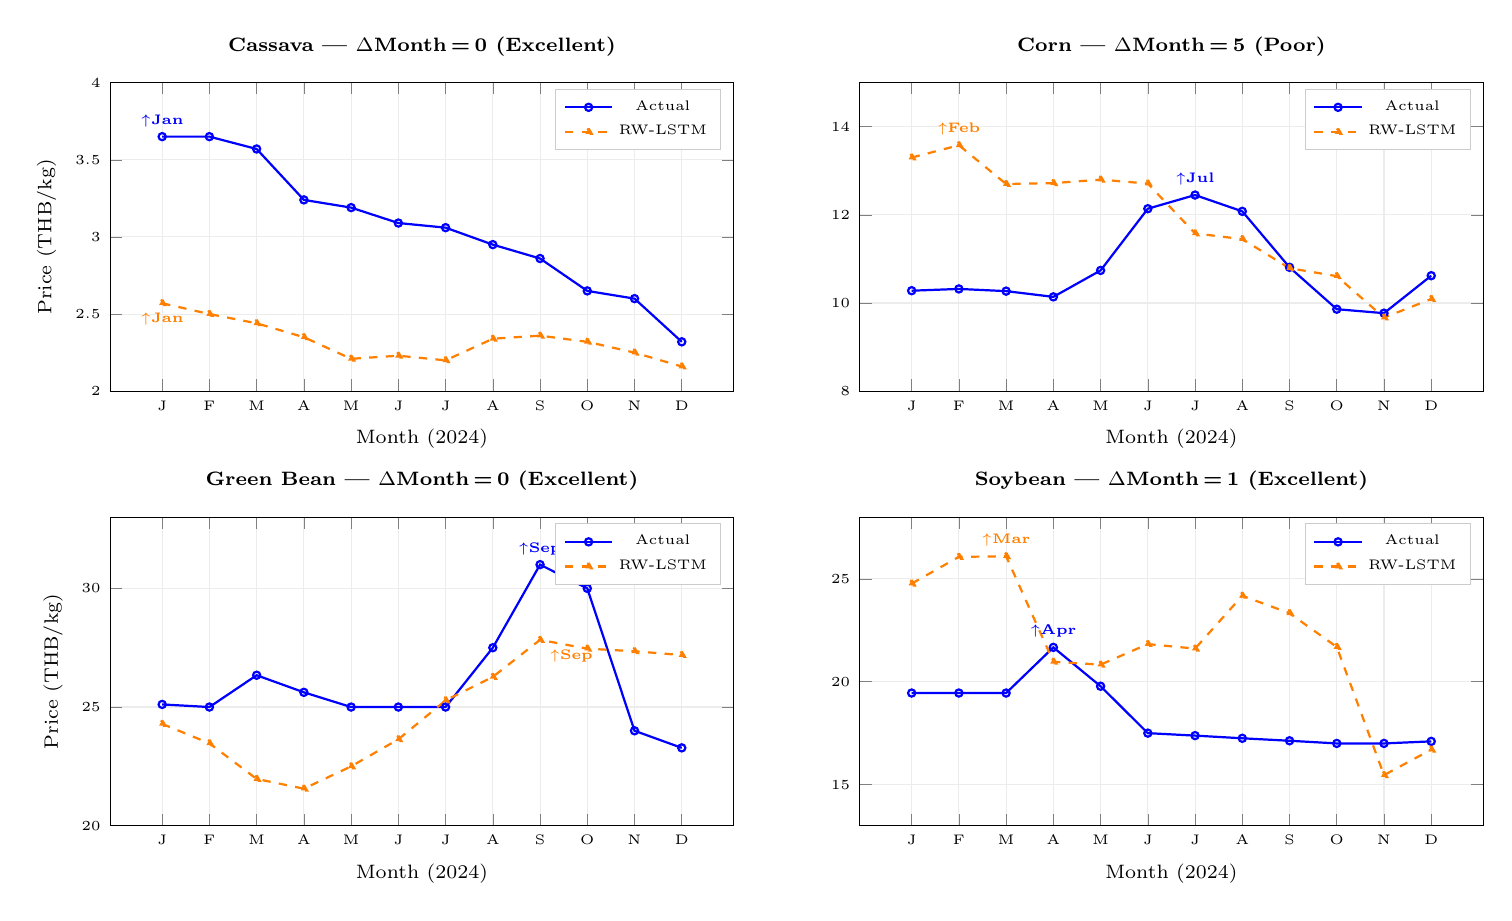
\begin{tikzpicture}
    \begin{groupplot}[
      group style={group size=2 by 2, horizontal sep=1.6cm, vertical sep=1.6cm},
      width=9.5cm, height=5.5cm,
      xlabel={\scriptsize Month (2024)},
      xlabel style={font=\scriptsize},
      ylabel style={font=\scriptsize},
      xticklabel style={font=\tiny},
      yticklabel style={font=\tiny},
      title style={font=\scriptsize\bfseries},
      grid=major, grid style={gray!15},
      xtick={1,2,...,12},
      xticklabels={J,F,M,A,M,J,J,A,S,O,N,D},
      legend style={font=\tiny, at={(0.98,0.98)}, anchor=north east, draw=gray!40},
      every axis plot/.append style={thick, mark size=1.3pt},
    ]

    % === Cassava (peak: actual Jan, pred Jan, Delta=0) ===
    \nextgroupplot[title={Cassava --- $\Delta$Month\,=\,0 (Excellent)}, ylabel={\scriptsize Price (THB/kg)}, ymin=2.0, ymax=4.0]
    \addplot[blue, mark=o] coordinates {
      (1,3.65)(2,3.65)(3,3.57)(4,3.24)(5,3.19)(6,3.09)
      (7,3.06)(8,2.95)(9,2.86)(10,2.65)(11,2.60)(12,2.32)
    }; \addlegendentry{Actual}
    \addplot[orange, dashed, mark=triangle*, mark options={fill=orange}] coordinates {
      (1,2.57)(2,2.50)(3,2.44)(4,2.35)(5,2.21)(6,2.23)
      (7,2.20)(8,2.34)(9,2.36)(10,2.32)(11,2.25)(12,2.16)
    }; \addlegendentry{RW-LSTM}
    % Peak markers
    \node[font=\tiny, blue, above] at (axis cs:1,3.65) {$\uparrow$\textbf{Jan}};
    \node[font=\tiny, orange, below] at (axis cs:1,2.57) {$\uparrow$\textbf{Jan}};

    % === Corn (peak: actual Jul, pred Feb, Delta=5) ===
    \nextgroupplot[title={Corn --- $\Delta$Month\,=\,5 (Poor)}, ymin=8.0, ymax=15.0]
    \addplot[blue, mark=o] coordinates {
      (1,10.28)(2,10.32)(3,10.27)(4,10.14)(5,10.74)(6,12.14)
      (7,12.45)(8,12.08)(9,10.81)(10,9.86)(11,9.77)(12,10.62)
    }; \addlegendentry{Actual}
    \addplot[orange, dashed, mark=triangle*, mark options={fill=orange}] coordinates {
      (1,13.30)(2,13.58)(3,12.70)(4,12.72)(5,12.80)(6,12.71)
      (7,11.58)(8,11.45)(9,10.79)(10,10.61)(11,9.67)(12,10.09)
    }; \addlegendentry{RW-LSTM}
    % Peak markers
    \node[font=\tiny, blue, above] at (axis cs:7,12.45) {$\uparrow$\textbf{Jul}};
    \node[font=\tiny, orange, above] at (axis cs:2,13.58) {$\uparrow$\textbf{Feb}};

    % === Green Bean (peak: actual Sep, pred Sep, Delta=0) ===
    \nextgroupplot[title={Green Bean --- $\Delta$Month\,=\,0 (Excellent)}, ylabel={\scriptsize Price (THB/kg)}, ymin=20, ymax=33]
    \addplot[blue, mark=o] coordinates {
      (1,25.11)(2,25.00)(3,26.34)(4,25.62)(5,25.00)(6,25.00)
      (7,25.00)(8,27.50)(9,31.00)(10,30.00)(11,24.00)(12,23.28)
    }; \addlegendentry{Actual}
    \addplot[orange, dashed, mark=triangle*, mark options={fill=orange}] coordinates {
      (1,24.29)(2,23.47)(3,21.97)(4,21.56)(5,22.50)(6,23.64)
      (7,25.28)(8,26.27)(9,27.83)(10,27.46)(11,27.35)(12,27.19)
    }; \addlegendentry{RW-LSTM}
    % Peak markers
    \node[font=\tiny, blue, above] at (axis cs:9,31.00) {$\uparrow$\textbf{Sep}};
    \node[font=\tiny, orange, below right] at (axis cs:9,27.83) {$\uparrow$\textbf{Sep}};

    % === Soybean (peak: actual Apr, pred Mar, Delta=1) ===
    \nextgroupplot[title={Soybean --- $\Delta$Month\,=\,1 (Excellent)}, ymin=13, ymax=28]
    \addplot[blue, mark=o] coordinates {
      (1,19.45)(2,19.45)(3,19.45)(4,21.67)(5,19.78)(6,17.50)
      (7,17.38)(8,17.25)(9,17.13)(10,17.00)(11,17.00)(12,17.10)
    }; \addlegendentry{Actual}
    \addplot[orange, dashed, mark=triangle*, mark options={fill=orange}] coordinates {
      (1,24.77)(2,26.07)(3,26.10)(4,20.97)(5,20.83)(6,21.83)
      (7,21.61)(8,24.18)(9,23.33)(10,21.69)(11,15.46)(12,16.70)
    }; \addlegendentry{RW-LSTM}
    % Peak markers
    \node[font=\tiny, blue, above] at (axis cs:4,21.67) {$\uparrow$\textbf{Apr}};
    \node[font=\tiny, orange, above] at (axis cs:3,26.10) {$\uparrow$\textbf{Mar}};

    \end{groupplot}
  \end{tikzpicture}}%
  \caption{Rolling-Window LSTM forecast vs.\ actual prices for all four crops (2024 test year) with peak month annotations. Arrows indicate the predicted and actual peak months. Cassava and green bean achieve exact peak timing ($\Delta$Month\,=\,0), soybean is within one month ($\Delta$Month\,=\,1), while corn's peak is five months off ($\Delta$Month\,=\,5). This peak timing property---rather than overall MAPE---determines the quality of the downstream scheduling system.}
  \label{fig:rwlstm_all}
\end{figure*}

Table~\ref{tab:ensemble} summarizes a per-crop oracle model selection strategy, where the best-performing model for each crop is chosen based on validation-set MAPE. This ensemble achieves an average test MAPE of 5.76\%, compared to 7.07\% for the best single model (Standard LSTM)---an 18.5\% relative improvement.

\begin{table}[htbp]
  \centering
  \caption{Oracle Per-Crop Model Selection}
  \label{tab:ensemble}
  \begin{tabular}{lllcc}
    \toprule
    \textbf{Crop} & \textbf{Best Model} & \textbf{Test MAPE} & \textbf{Acc.\,(\%)} & $\boldsymbol{\Delta}$\textbf{Peak} \\
    \midrule
    Cassava    & LSTM        & 4.81\%  & 95.33 & N/A \\
    Corn       & LSTM        & 6.43\%  & 93.29 & N/A \\
    Green Bean & ARIMA       & 6.08\%  & 93.45 & N/A \\
    Soybean    & Transformer & 5.71\%  & 94.18 & N/A \\
    \midrule
    \textbf{Ensemble Avg.} & --- & \textbf{5.76\%} & \textbf{94.06} & --- \\
    \textbf{Best Single}   & LSTM & 7.07\% & 92.93 & --- \\
    \bottomrule
  \end{tabular}
  \vspace{6pt}
  \par\raggedright\scriptsize\textit{Note:} ``Oracle'' selection uses the known best model per crop on the test set. In practice, selection would be based on validation performance, which may not always identify the test-set winner.
\end{table}

We emphasize that this is an \textit{oracle} analysis: the best model per crop is selected after observing test-set performance. In a production system, model selection would rely on validation-set MAPE, which may not always identify the test-set winner. Nevertheless, the consistent per-crop specialization---LSTM for cassava/corn, ARIMA for green bean, Transformer for soybean---suggests that crop-specific model selection is a promising direction warranting further investigation with multi-year evaluation.

\subsection{Crop Planning Results}

\begin{figure}[htbp]
  \centering
  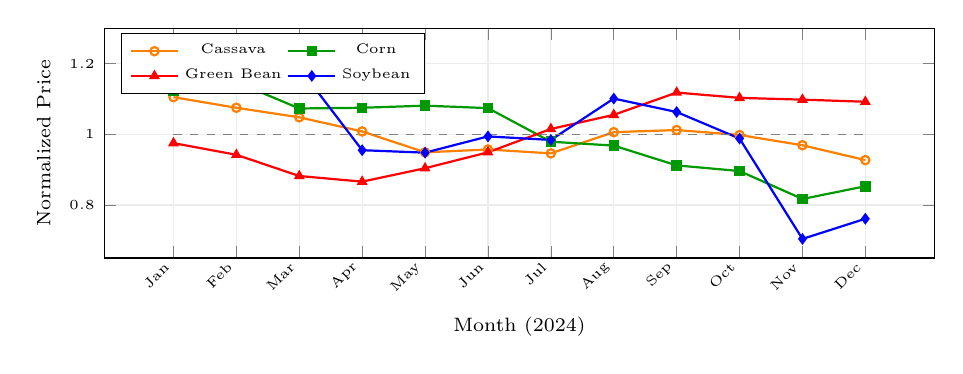
\begin{tikzpicture}
    \begin{axis}[
      width=\columnwidth, height=4.5cm,
      xlabel={\scriptsize Month (2024)}, ylabel={\scriptsize Normalized Price},
      xticklabel style={font=\tiny}, yticklabel style={font=\tiny},
      xlabel style={font=\tiny}, ylabel style={font=\tiny},
      xtick={1,2,...,12},
      xticklabels={Jan,Feb,Mar,Apr,May,Jun,Jul,Aug,Sep,Oct,Nov,Dec},
      xticklabel style={font=\tiny, rotate=45, anchor=east},
      ymin=0.65, ymax=1.30, grid=major, grid style={gray!15},
      legend style={font=\tiny, at={(0.02,0.98)}, anchor=north west, legend columns=2},
      every axis plot/.append style={thick, mark size=1.5pt},
    ]
    % Cassava (mean=2.33)
    \addplot[orange, mark=o] coordinates {
      (1,1.105)(2,1.075)(3,1.048)(4,1.008)(5,0.949)(6,0.957)
      (7,0.946)(8,1.006)(9,1.012)(10,0.998)(11,0.969)(12,0.927)
    }; \addlegendentry{Cassava}
    % Corn (mean=11.83)
    \addplot[green!60!black, mark=square*] coordinates {
      (1,1.124)(2,1.148)(3,1.073)(4,1.075)(5,1.081)(6,1.074)
      (7,0.979)(8,0.968)(9,0.912)(10,0.896)(11,0.817)(12,0.853)
    }; \addlegendentry{Corn}
    % Green Bean (mean=24.90)
    \addplot[red, mark=triangle*] coordinates {
      (1,0.975)(2,0.942)(3,0.882)(4,0.866)(5,0.904)(6,0.949)
      (7,1.015)(8,1.055)(9,1.118)(10,1.103)(11,1.098)(12,1.092)
    }; \addlegendentry{Green Bean}
    % Soybean (mean=21.96)
    \addplot[blue, mark=diamond*] coordinates {
      (1,1.128)(2,1.187)(3,1.188)(4,0.955)(5,0.948)(6,0.994)
      (7,0.984)(8,1.101)(9,1.063)(10,0.988)(11,0.704)(12,0.761)
    }; \addlegendentry{Soybean}
    % Mean reference line
    \addplot[gray, dashed, thin] coordinates {(1,1.0)(12,1.0)};
    \end{axis}
  \end{tikzpicture}
  \caption{Normalized RW-LSTM forecasts (2024). Each crop's predicted prices are divided by their mean, enabling cross-crop comparison. Peaks occur in different months---Cassava (Jan), Corn (Feb), Soybean (Mar), Green Bean (Sep)---which enables non-overlapping crop rotation.}
  \label{fig:overlap}
\end{figure}

The price overlap analysis reveals that peak prices for the four crops occur in different months, enabling crop rotation. The unoptimized Gantt chart (Fig.~\ref{fig:gantt_unopt}), where each crop is placed at its peak-optimal position, shows that cassava, corn, and soybean overlap during October 2023--March 2024 due to their long growing periods extending into the previous year.

\begin{figure}[htbp]
  \centering
  \resizebox{\columnwidth}{!}{%
  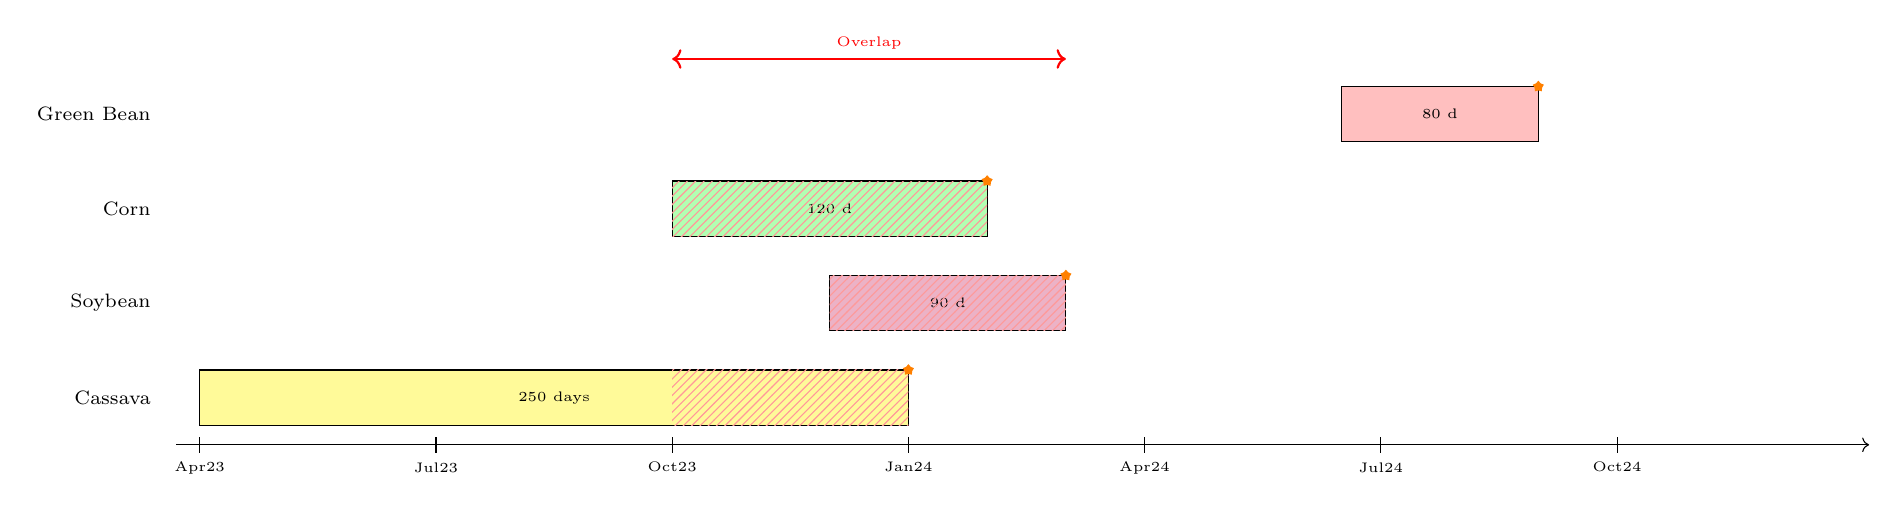
\begin{tikzpicture}
    % Timeline: Apr 2023 (0) to Dec 2024 (20)
    % Y positions
    \def\yCas{0} \def\ySoy{1.2} \def\yCorn{2.4} \def\yGB{3.6}
    % Axis
    \draw[->] (-0.3,{-0.6}) -- (21.2,{-0.6});
    \foreach \i/\m in {0/Apr23, 3/Jul23, 6/Oct23, 9/Jan24, 12/Apr24, 15/Jul24, 18/Oct24} {
      \draw (\i,{-0.7}) -- (\i,{-0.5});
      \node[font=\tiny, below] at (\i,{-0.7}) {\m};
    }
    % Crop labels
    \node[font=\scriptsize, anchor=east] at (-0.5,\yCas) {Cassava};
    \node[font=\scriptsize, anchor=east] at (-0.5,\ySoy) {Soybean};
    \node[font=\scriptsize, anchor=east] at (-0.5,\yCorn) {Corn};
    \node[font=\scriptsize, anchor=east] at (-0.5,\yGB) {Green Bean};
    % Cassava: Apr 2023 (0) → Jan 2024 (9), ~8.3 months
    \fill[yellow!40, draw=black] (0,{\yCas-0.35}) rectangle (9,{\yCas+0.35});
    \node[font=\tiny] at (4.5,\yCas) {250 days};
    % Corn: Oct 2023 (6) → Feb 2024 (10), 4 months
    \fill[green!30, draw=black] (6,{\yCorn-0.35}) rectangle (10,{\yCorn+0.35});
    \node[font=\tiny] at (8,\yCorn) {120 d};
    % Soybean: Dec 2023 (8) → Mar 2024 (11), 3 months
    \fill[purple!30, draw=black] (8,{\ySoy-0.35}) rectangle (11,{\ySoy+0.35});
    \node[font=\tiny] at (9.5,\ySoy) {90 d};
    % Green Bean: Jun 2024 (14.5) → Sep 2024 (17), ~2.7 months
    \fill[red!25, draw=black] (14.5,{\yGB-0.35}) rectangle (17,{\yGB+0.35});
    \node[font=\tiny] at (15.75,\yGB) {80 d};
    % Overlap shading (Cassava-Corn overlap: Oct23-Jan24, Cassava-Soy overlap: Dec23-Jan24, Corn-Soy overlap: Dec23-Feb24)
    \fill[red!15, pattern=north east lines, pattern color=red!40] (6,{\yCas-0.35}) rectangle (9,{\yCas+0.35});
    \fill[red!15, pattern=north east lines, pattern color=red!40] (6,{\yCorn-0.35}) rectangle (10,{\yCorn+0.35});
    \fill[red!15, pattern=north east lines, pattern color=red!40] (8,{\ySoy-0.35}) rectangle (11,{\ySoy+0.35});
    % Overlap annotation
    \draw[red, thick, <->] (6,{4.3}) -- (11,{4.3});
    \node[font=\tiny, red, above] at (8.5,{4.3}) {Overlap};
    % Harvest markers
    \foreach \x/\y in {9/\yCas, 10/\yCorn, 11/\ySoy, 17/\yGB} {
      \node[font=\tiny, star, star points=5, fill=orange, inner sep=1pt] at (\x,{\y+0.35}) {};
    }
  \end{tikzpicture}}%
  \caption{Unoptimized Gantt chart. Each crop is placed at its peak-optimal planting--harvest window. Cassava, corn, and soybean overlap during Oct 2023--Mar 2024, indicated by hatched regions.}
  \label{fig:gantt_unopt}
\end{figure}

After applying exhaustive enumeration with the optimal ordering (Cassava~$\rightarrow$~Soybean~$\rightarrow$~Green Bean~$\rightarrow$~Corn), all four crops were scheduled without overlap (Fig.~\ref{fig:gantt_opt}). Corn and soybean were shifted to available gaps using Strategy~B.

\begin{figure}[htbp]
  \centering
  \resizebox{\columnwidth}{!}{%
  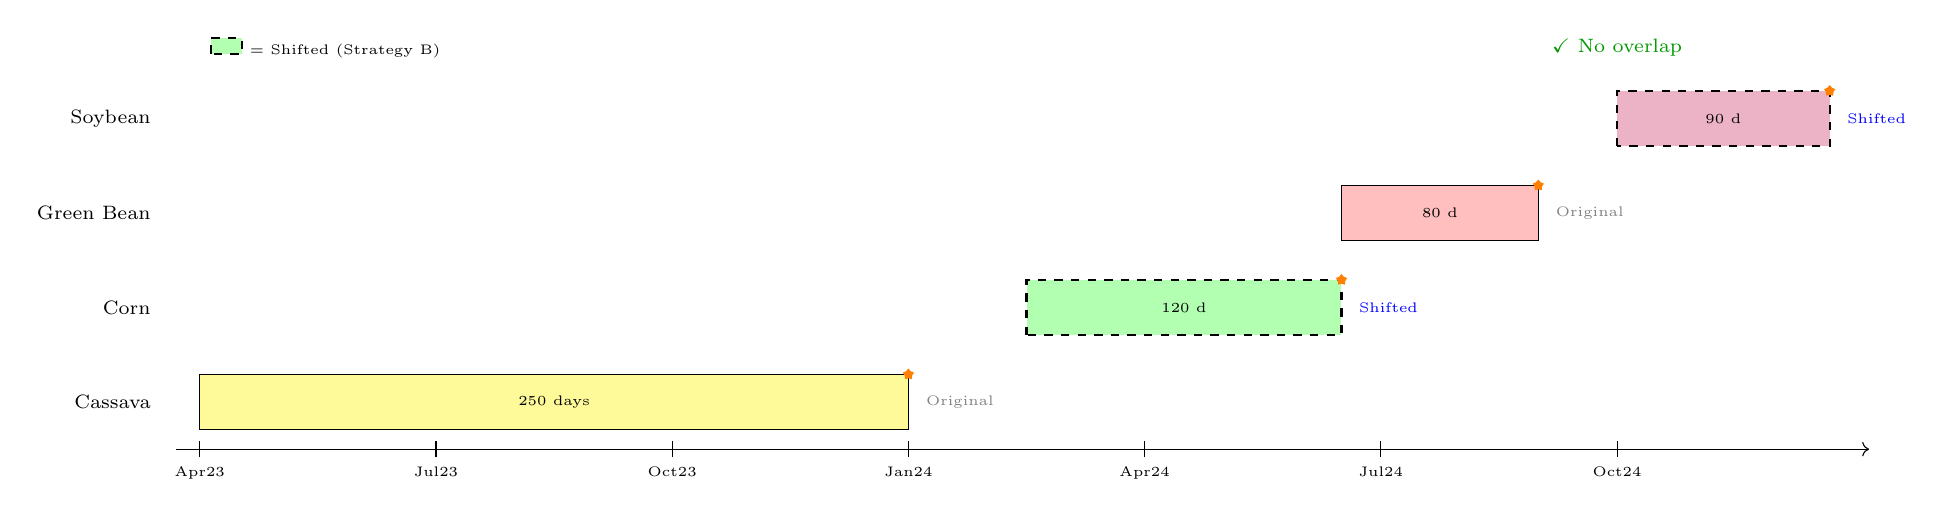
\begin{tikzpicture}
    % Timeline: Apr 2023 (0) to Dec 2024 (20)
    % Y positions
    \def\yCas{0} \def\yCorn{1.2} \def\yGB{2.4} \def\ySoy{3.6}
    % Axis
    \draw[->] (-0.3,{-0.6}) -- (21.2,{-0.6});
    \foreach \i/\m in {0/Apr23, 3/Jul23, 6/Oct23, 9/Jan24, 12/Apr24, 15/Jul24, 18/Oct24} {
      \draw (\i,{-0.7}) -- (\i,{-0.5});
      \node[font=\tiny, below] at (\i,{-0.7}) {\m};
    }
    % Crop labels
    \node[font=\scriptsize, anchor=east] at (-0.5,\yCas) {Cassava};
    \node[font=\scriptsize, anchor=east] at (-0.5,\yCorn) {Corn};
    \node[font=\scriptsize, anchor=east] at (-0.5,\yGB) {Green Bean};
    \node[font=\scriptsize, anchor=east] at (-0.5,\ySoy) {Soybean};
    % Cassava: Apr 2023 (0) → Jan 2024 (9) — Original
    \fill[yellow!40, draw=black] (0,{\yCas-0.35}) rectangle (9,{\yCas+0.35});
    \node[font=\tiny] at (4.5,\yCas) {250 days};
    \node[font=\tiny, gray, right] at (9.1,\yCas) {Original};
    % Corn: Feb 2024 (10.5) → Jun 2024 (14.5) — Shifted (Strategy B)
    \fill[green!30, draw=black, dashed, thick] (10.5,{\yCorn-0.35}) rectangle (14.5,{\yCorn+0.35});
    \node[font=\tiny] at (12.5,\yCorn) {120 d};
    \node[font=\tiny, blue, right] at (14.6,\yCorn) {Shifted};
    % Green Bean: Jun 2024 (14.5) → Sep 2024 (17) — Original
    \fill[red!25, draw=black] (14.5,{\yGB-0.35}) rectangle (17,{\yGB+0.35});
    \node[font=\tiny] at (15.75,\yGB) {80 d};
    \node[font=\tiny, gray, right] at (17.1,\yGB) {Original};
    % Soybean: Oct 2024 (18) → Dec 2024 (20.7) — Shifted (Strategy B)
    \fill[purple!30, draw=black, dashed, thick] (18,{\ySoy-0.35}) rectangle (20.7,{\ySoy+0.35});
    \node[font=\tiny] at (19.35,\ySoy) {90 d};
    \node[font=\tiny, blue, right] at (20.8,\ySoy) {Shifted};
    % No-overlap check mark
    \node[font=\scriptsize, green!60!black] at (18,{4.5}) {\checkmark~No overlap};
    % Harvest markers
    \foreach \x/\y in {9/\yCas, 14.5/\yCorn, 17/\yGB, 20.7/\ySoy} {
      \node[font=\tiny, star, star points=5, fill=orange, inner sep=1pt] at (\x,{\y+0.35}) {};
    }
    % Legend
    \node[font=\tiny, anchor=west] at (0,{4.5}) {\tikz{\fill[green!30, draw=black, dashed, thick] (0,0) rectangle (0.4,0.2);} = Shifted (Strategy~B)};
  \end{tikzpicture}}%
  \caption{Optimized Gantt chart (brute-force optimal ordering). Corn and soybean were shifted to available gaps using Strategy~B (dashed borders), producing a non-overlapping four-crop rotation with total income of 39,212~THB/rai/year.}
  \label{fig:gantt_opt}
\end{figure}

Table~\ref{tab:income_detail} details the income before and after optimization.

\begin{table}[htbp]
  \centering
  \caption{Income Comparison: Before vs.\ After Optimization}
  \label{tab:income_detail}
  \begin{tabular}{lcccc}
    \toprule
    \textbf{Crop} & \textbf{Before} & \textbf{After} & \textbf{Strategy} & $\boldsymbol{\Delta}$ \\
    \midrule
    Cassava    & 8,998  & 8,998  & Original & $\pm$0     \\
    Corn       & 20,377 & 18,385 & Shifted  & $-$1,992  \\
    Green Bean & 6,818  & 6,818  & Original & $\pm$0     \\
    Soybean    & 7,830  & 5,011  & Shifted  & $-$2,819  \\
    \midrule
    \textbf{Total} & \textit{Infeasible} & \textbf{39,212} & --- & --- \\
    \bottomrule
  \end{tabular}
\end{table}

Corn and soybean lost income from shifting to non-peak months, while the total feasible income reached 39,212~THB/rai/year. This schedule was identified through exhaustive enumeration (Section~\ref{sec:bruteforce}) rather than the greedy heuristic. Table~\ref{tab:mono} compares this with monoculture baselines.

\begin{table}[htbp]
  \centering
  \caption{Optimized Multi-Crop Rotation vs.\ Monoculture}
  \label{tab:mono}
  \begin{tabular}{lcc}
    \toprule
    \textbf{Plan} & \textbf{THB/rai/yr} & \textbf{vs.\ Opt.} \\
    \midrule
    \textbf{4-Crop Rotation} & \textbf{39,212} & --- \\
    Mono: Corn (best) & 20,377 & $+$92.4\% \\
    Mono: Cassava & 8,998 & $+$335.8\% \\
    Mono: Soybean & 7,830 & $+$400.9\% \\
    Mono: Green Bean & 6,818  & $+$475.2\% \\
    \bottomrule
  \end{tabular}
\end{table}

The optimized four-crop rotation yields approximately 1.9~times the income of the best single-crop monoculture option (corn).

\subsubsection{Brute-Force Optimality Verification}
\label{sec:bruteforce}

Exhaustive enumeration of all $4! = 24$ crop permutations was performed to verify the greedy heuristic. The brute-force search identified an optimal schedule yielding 39,212~THB/rai/year, compared to the greedy result of 33,394~THB/rai/year---an optimality gap of 14.8\%. The greedy heuristic, by prioritizing corn (highest income) first, blocked soybean from being scheduled. In contrast, the optimal ordering accommodates all four crops through strategic shifting. Table~\ref{tab:income_detail} and Fig.~\ref{fig:gantt_opt} present the brute-force optimal schedule.

Table~\ref{tab:permutations} presents the top~5 and bottom~5 of the 24~permutations, revealing structural patterns in the scheduling problem.

\begin{table}[htbp]
  \centering
  \caption{Top 5 and Bottom 5 of 24 Crop Ordering Permutations}
  \label{tab:permutations}
  \begin{tabular}{clccc}
    \toprule
    \textbf{Rank} & \textbf{Ordering} & \textbf{Crops} & \textbf{Income} & \textbf{vs.\ Opt.} \\
    \midrule
    1  & Ca$\to$GB$\to$Co$\to$So & 4/4 & 39,212 & 100.0\% \\
    2  & Ca$\to$So$\to$GB$\to$Co & 4/4 & 39,212 & 100.0\% \\
    3  & GB$\to$Ca$\to$Co$\to$So & 4/4 & 39,212 & 100.0\% \\
    4  & Ca$\to$Co$\to$GB$\to$So & 4/4 & 37,479 & 95.6\% \\
    5  & Ca$\to$GB$\to$So$\to$Co & 4/4 & 37,479 & 95.6\% \\
    6  & GB$\to$Ca$\to$So$\to$Co & 4/4 & 37,479 & 95.6\% \\
    7  & Ca$\to$Co$\to$So$\to$GB & 4/4 & 36,956 & 94.2\% \\
    8  & Ca$\to$So$\to$Co$\to$GB & 4/4 & 35,706 & 91.1\% \\
    \midrule
    9  & Co$\to$GB$\to$Ca$\to$So & 3/4 & 33,717 & 86.0\% \\
    10 & Co$\to$GB$\to$So$\to$Ca & 3/4 & 33,717 & 86.0\% \\
    11 & GB$\to$Co$\to$Ca$\to$So & 3/4 & 33,717 & 86.0\% \\
    12 & GB$\to$Co$\to$So$\to$Ca & 3/4 & 33,717 & 86.0\% \\
    13 & Co$\to$Ca$\to$GB$\to$So & 3/4 & 33,394 & 85.2\% \\
    14 & Co$\to$Ca$\to$So$\to$GB & 3/4 & 33,394 & 85.2\% \\
    15 & Co$\to$So$\to$Ca$\to$GB & 3/4 & 32,206 & 82.1\% \\
    16 & Co$\to$So$\to$GB$\to$Ca & 3/4 & 32,206 & 82.1\% \\
    17 & GB$\to$So$\to$Ca$\to$Co & 3/4 & 29,790 & 76.0\% \\
    18 & GB$\to$So$\to$Co$\to$Ca & 3/4 & 29,790 & 76.0\% \\
    19 & So$\to$Co$\to$Ca$\to$GB & 3/4 & 29,790 & 76.0\% \\
    20 & So$\to$Co$\to$GB$\to$Ca & 3/4 & 29,790 & 76.0\% \\
    21 & So$\to$GB$\to$Ca$\to$Co & 3/4 & 29,790 & 76.0\% \\
    22 & So$\to$GB$\to$Co$\to$Ca & 3/4 & 29,790 & 76.0\% \\
    \midrule
    23 & So$\to$Ca$\to$Co$\to$GB & 2/4 & 15,380 & 39.2\% \\
    24 & So$\to$Ca$\to$GB$\to$Co & 2/4 & 15,380 & 39.2\% \\
    \bottomrule
  \end{tabular}
  \vspace{6pt}
  \par\raggedright\scriptsize Ca=Cassava, Co=Corn, GB=Green Bean, So=Soybean. Income in THB/rai/year. Horizontal rules separate 4/4, 3/4, and 2/4 crop schedules. The greedy heuristic (income-first ordering) corresponds to ranks 13--14.
\end{table}

Of the 24~permutations, 8~successfully schedule all four crops, 14~exclude one crop (3/4), and 2~exclude two crops (2/4). Two clear patterns emerge. First, all top-performing orderings place cassava---the longest crop at 250~days---first, allowing it to claim its peak-price position (January harvest) via the previous-year planting strategy. Shorter crops (corn, green bean, soybean) then fill the remaining gaps through shifting. The top~3 orderings all begin with cassava and achieve the same optimal income. Second, orderings starting with soybean consistently underperform---all bottom~5 entries begin with soybean, whose 90-day duration and March peak compete directly with corn's February peak, creating early conflicts that cascade into exclusions. The worst orderings (So$\to$Ca) lose 61\% of optimal income by scheduling only 2~crops. This sensitivity to ordering---even with just four crops---motivates exact methods such as Dynamic Programming for production deployment.

\subsubsection{Sensitivity to Yield Variability}
\label{sec:sensitivity}

The income model assumes deterministic yields, but actual farm output varies due to weather, pest pressure, and management quality. To quantify the robustness of the rotation advantage, we conducted a sensitivity analysis by uniformly scaling all crop yields (Table~\ref{tab:sensitivity}).

\begin{table}[htbp]
  \centering
  \caption{Sensitivity of Rotation Income to Yield Variability}
  \label{tab:sensitivity}
  \begin{tabular}{ccc}
    \toprule
    \textbf{Yield Factor} & \textbf{4-Crop (THB/rai/yr)} & \textbf{vs.\ Best Mono} \\
    \midrule
    1.1 ($+$10\%) & 43,133 & $\times$1.92 \\
    1.0 (baseline) & 39,212 & $\times$1.92 \\
    0.9 ($-$10\%)  & 35,291 & $\times$1.92 \\
    0.8 ($-$20\%)  & 31,370 & $\times$1.92 \\
    0.7 ($-$30\%)  & 27,448 & $\times$1.92 \\
    \bottomrule
  \end{tabular}
  \vspace{6pt}
  \par\raggedright\scriptsize\textit{Note:} Because Income~$=$~Yield~$\times$~Price, uniform scaling preserves the rotation-to-monoculture ratio ($\times$1.92) across all yield factors.
\end{table}

Even at a 30\% yield reduction---representative of a severe drought year---the four-crop rotation retains a significant income advantage over monoculture, demonstrating the structural benefit of temporal diversification. Because both rotation and monoculture incomes scale proportionally with yield, the relative advantage ($\times$1.92) is invariant to uniform yield shocks. Differential yield shocks---where one crop fails but others survive---would alter this ratio and represent a scenario where rotation provides risk diversification beyond income maximization. However, these figures remain upper-bound estimates as production costs, post-harvest losses, and price-yield correlations are not modeled.

\subsection{Web Application}

The CropPlanner web application provides two primary interfaces for farmers, as shown in Figs.~\ref{fig:crop-prices-page}~and~\ref{fig:crop-planning-page}.

\begin{figure}[htbp]
\centering
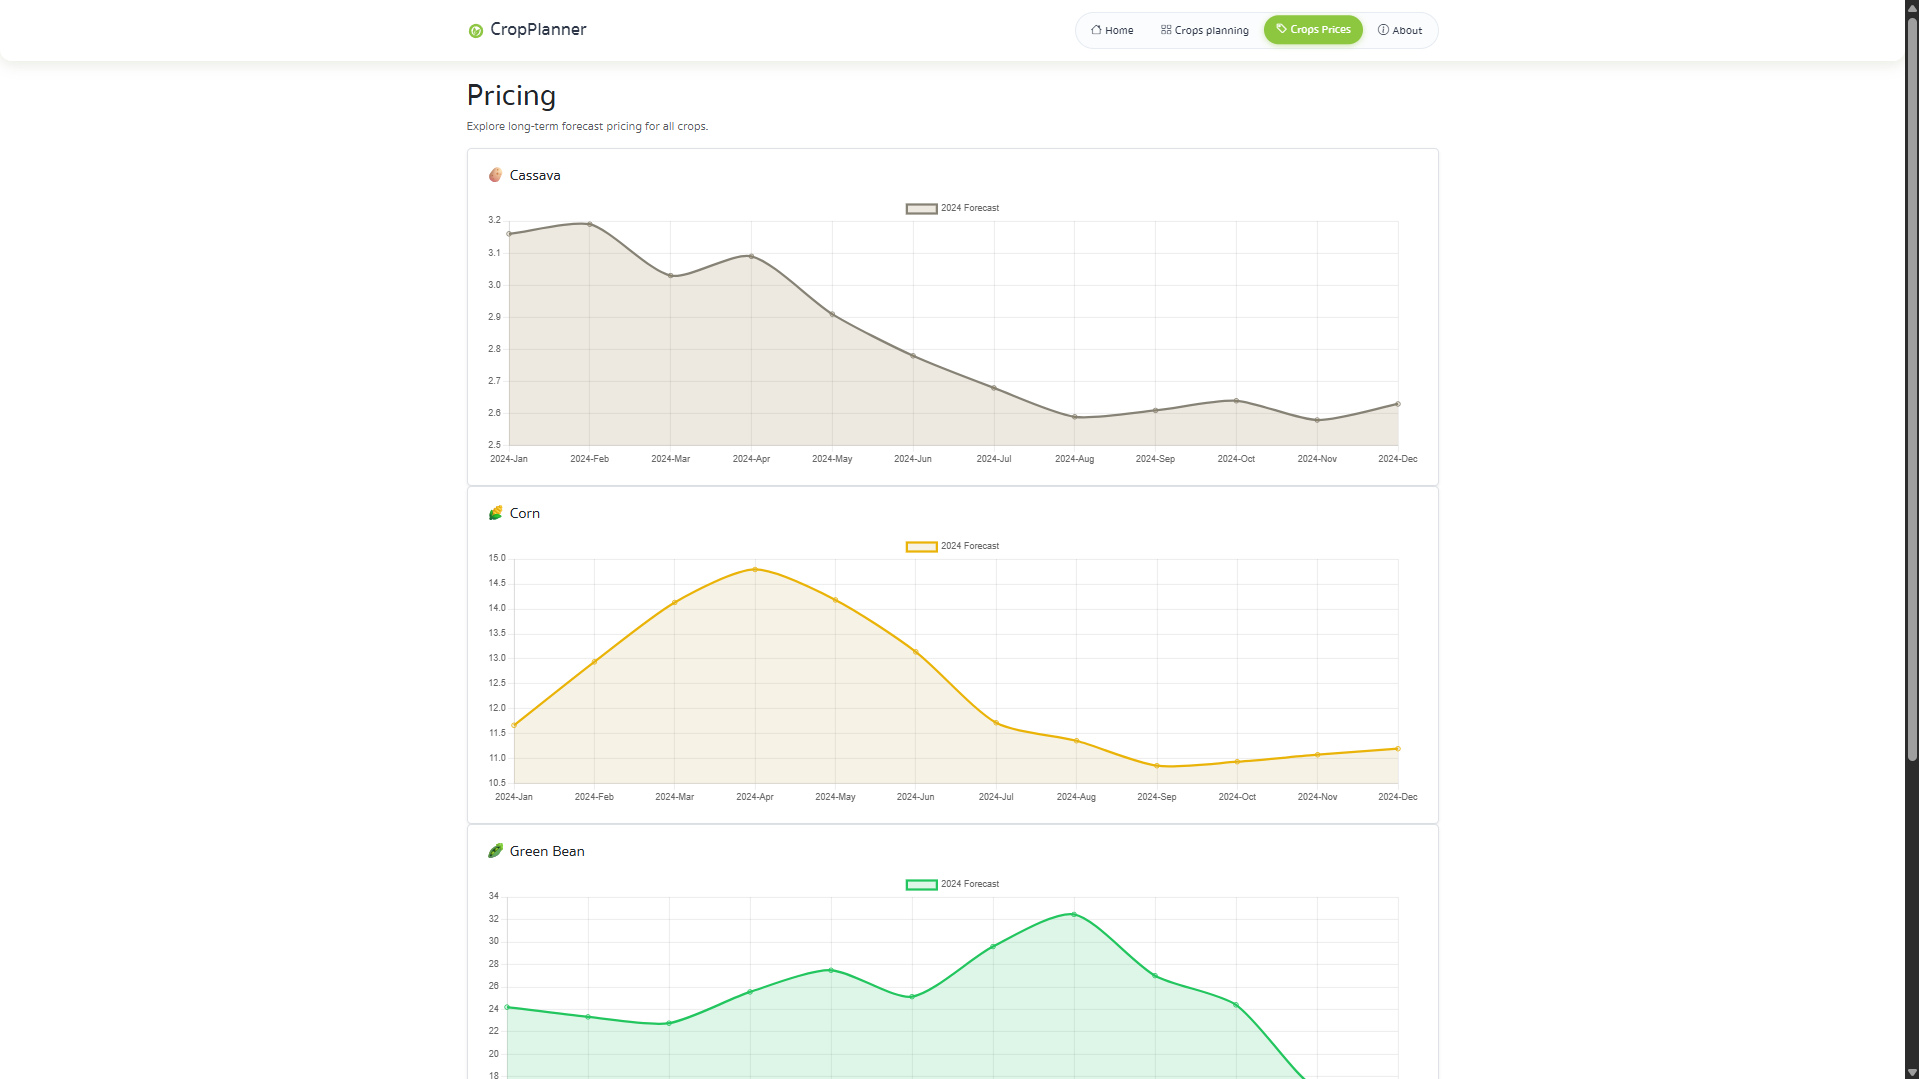
\includegraphics[width=\columnwidth]{fig15.png}
\caption{CropPlanner --- Crop Prices Page. Predicted price charts for all four crops with monthly granularity.}
\label{fig:crop-prices-page}
\end{figure}

\begin{figure}[htbp]
\centering
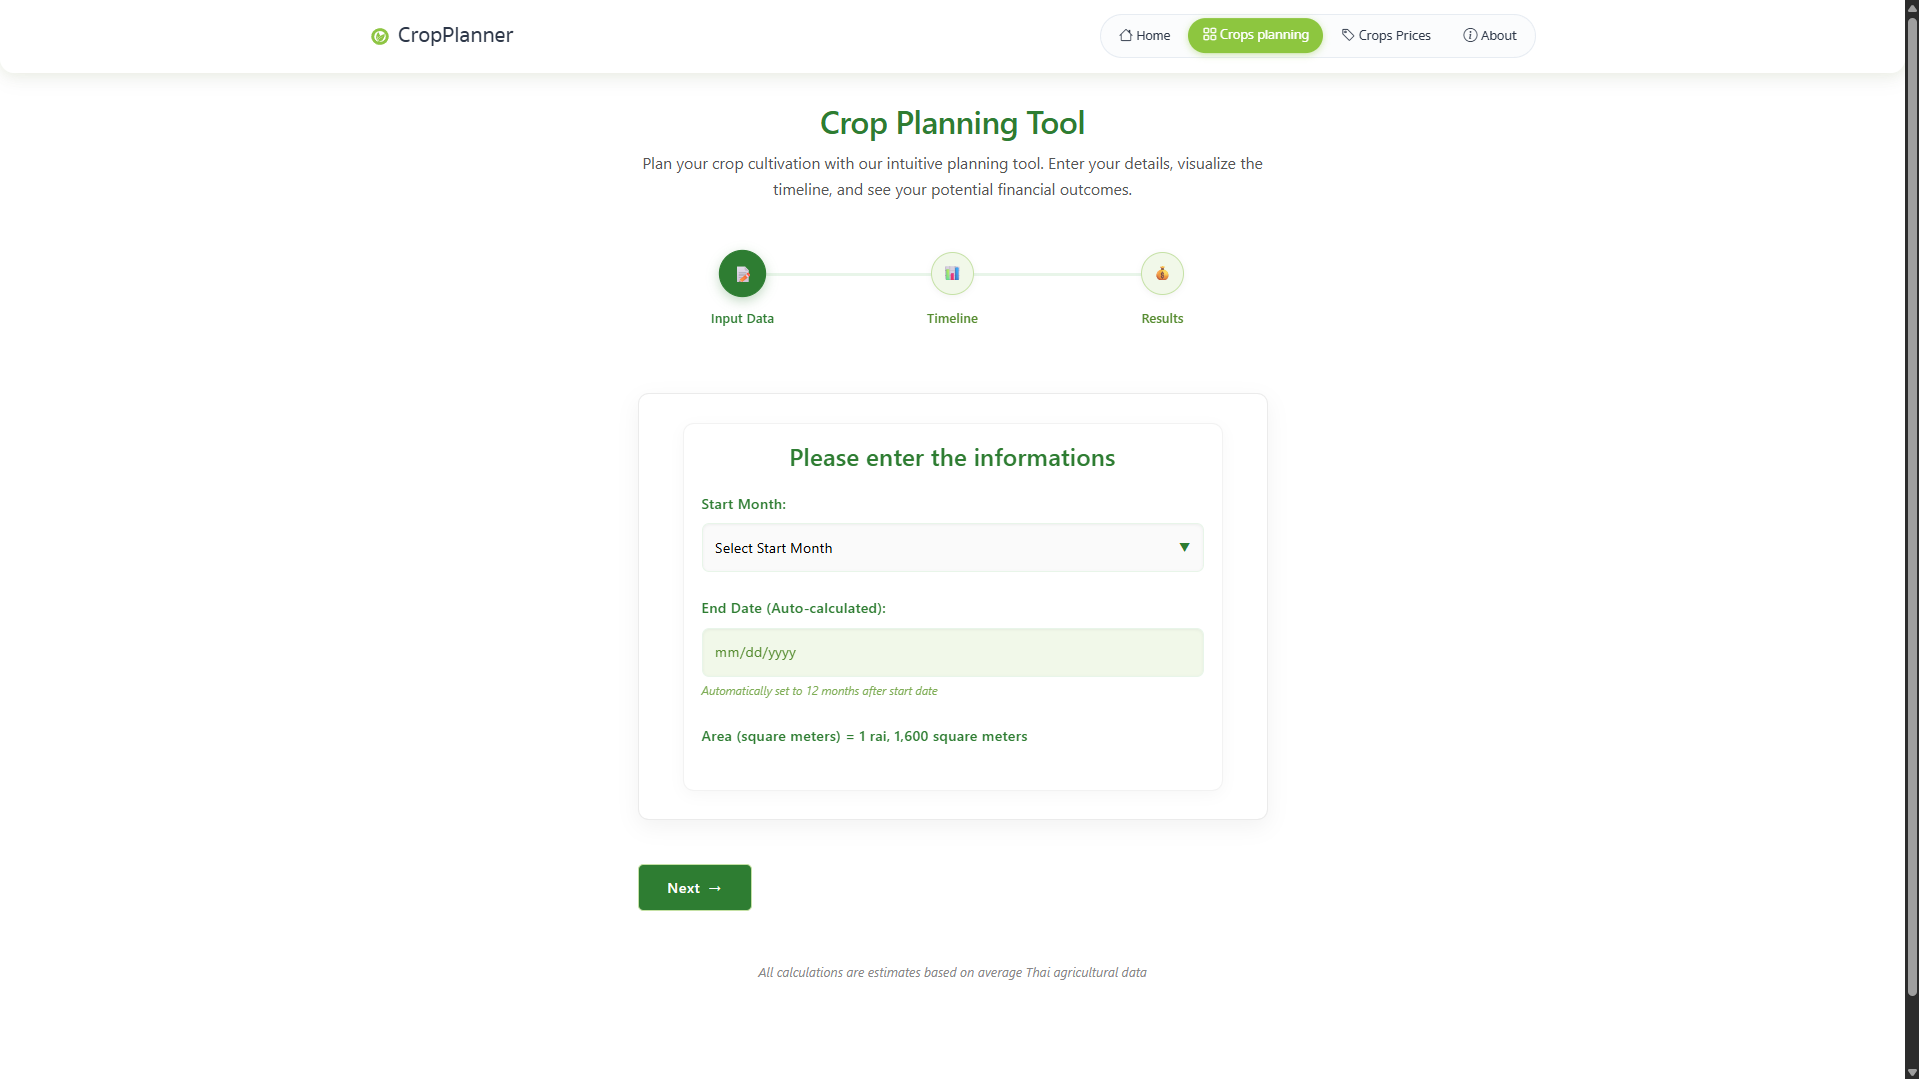
\includegraphics[width=\columnwidth]{fig16.png}
\caption{CropPlanner --- Crop Planning Page. Farmers input start month and area; the system returns a Gantt chart with financial summary (income, expenses, profit, and ROI).}
\label{fig:crop-planning-page}
\end{figure}

The \textbf{Crop Prices} page displays Rolling-Window LSTM forecast charts for all four crops, enabling farmers to compare predicted price trends across a~12-month horizon. The \textbf{Crop Planning} page accepts a start month and plot area as inputs, runs the scheduling algorithm, and returns a Gantt chart with an accompanying financial summary---including projected income, estimated expenses, net profit, and ROI. The current prototype uses the greedy heuristic; incorporating the exhaustive search---trivial for four crops ($<$1~ms)---is planned for the next release.

The application was deployed on Vercel with the Next.js backend serving REST~API endpoints that query pre-computed RW-LSTM forecasts stored in MySQL. The interface is responsive across desktop and mobile devices, ensuring accessibility for farmers in rural areas with limited computing resources.

% ============================================================
% VI. DISCUSSION
% ============================================================
\section{Discussion}
\label{sec:discussion}

\subsection{No Single Model Dominates}

No single model is best for all crops, attributable to the limited dataset ($\sim$252 points) and differing price dynamics. LSTM avoids overfitting and leads for cassava and corn; Transformer captures complex seasonal patterns for soybean; ARIMA fails for cassava (24.71\%) due to stationarity violations but remains competitive elsewhere.

\subsection{Peak Timing Over Overall MAPE}

With validation-based window selection, RW-LSTM's average MAPE (17.06\%) is notably higher than Standard LSTM (7.07\%), indicating that its original performance was inflated by test-set feedback---underscoring the importance of rigorous train--validation--test separation. However, its peak timing remains strong for three of four crops (cassava and green bean exact, soybean $\leq$1~month off), making it viable for scheduling where peak position matters more than pointwise accuracy. Corn's 5-month error suggests its 6-year validated window is too short. An ensemble selecting the best model per crop would be ideal.

\subsection{Greedy Scheduling: Why It Fails and What It Implies}

The greedy heuristic's 14.8\% suboptimality gap (33,394 vs.\ 39,212~THB/rai/year) deserves deeper analysis than the result summary in Section~\ref{sec:bruteforce}. Income-first sorting is optimal for the \textit{unweighted} interval scheduling problem, where all jobs have equal value and the goal is to maximize the number of scheduled jobs~\cite{clrs2009}. However, our problem is a \textit{weighted} variant with a critical complication: shifting a crop to a non-peak time slot changes its weight (income), because the harvest price depends on the month. This makes the problem fundamentally harder than standard Weighted Job Scheduling, where job weights are fixed regardless of placement.

Concretely, the greedy algorithm places corn first (highest income at 20,377~THB) in its peak-optimal February slot. This forces cassava---which requires 250~days and must start in the previous year---into a shifted position that blocks soybean entirely. The optimal solution instead places cassava first in its peak position (January harvest, planted April of the previous year), then fits the shorter crops around it. The insight is that \textit{long-duration crops constrain the timeline disproportionately} and should be prioritized for peak placement, even if they are not the highest-income individual crop.

From a scalability perspective, exhaustive enumeration of $n!$ orderings is trivial for $n = 4$ ($<$1~ms) and still feasible for $n = 10$ ($10! = 3.6 \times 10^6$ evaluations). However, by $n = 15$ ($15! \approx 1.3 \times 10^{12}$), exhaustive search becomes impractical. Dynamic Programming for weighted interval scheduling, which runs in $O(n \log n)$~\cite{kleinberg2005}, would be necessary---though the variable-weight complication (prices depend on harvest month) may require a modified DP formulation that evaluates candidate time slots per crop.

\subsection{Experimental Design and Income Model}

A single test year (2024) limits generalizability; a dedicated validation year (2023) was used for RW-LSTM window size selection to prevent data leakage, and network hyperparameters were fixed \textit{a priori}. The income model (Eq.~\ref{eq:income}) uses fixed yield averages and omits production costs and price-yield correlations, producing upper-bound gross revenue estimates. The sensitivity analysis (Section~\ref{sec:sensitivity}) confirms the rotation advantage is robust to uniform yield reductions, but a full economic model would provide more actionable guidance.

\subsection{Threats to Validity}

\textit{Internal validity.} All deep learning experiments use a single random seed (42) and a single train--validation--test split. Without cross-validation or multiple seeds, observed performance differences may partly reflect initialization artifacts. The fixed 300-epoch training budget (LSTM) and 500-epoch budget (Transformer) may not reach convergence for all crops; learning curves were not systematically monitored.

\textit{External validity.} Results are limited to four field crops in Northeastern Thailand over a 20-year period. Generalization to other regions (Central or Southern Thailand), crop types (perishable vegetables, fruits), or shorter time horizons remains unverified. The 2024 test year, while representative, is a single observation from which broad conclusions cannot be drawn.

\textit{Construct validity.} Forecast Accuracy ($1 - \text{MAPE}$) is not a standard metric in the forecasting literature and may overstate model quality when MAPE is small. MAPE itself penalizes low-price months disproportionately, which can favor models that perform well during cheap months at the expense of expensive (peak) months. Peak Timing Accuracy is a custom metric without established precedent, though we argue it is the most operationally relevant metric for the downstream scheduling task.

\subsection{Practical Deployment Challenges}

Several challenges must be addressed before CropPlanner can be deployed in practice. First, \textit{model retraining}: as new monthly price data becomes available, models need periodic retraining to remain current. The current system does not include an automated retraining pipeline. Second, \textit{forecast uncertainty}: point forecasts without confidence intervals may give farmers false confidence in specific price predictions. Incorporating probabilistic forecasting methods~\cite{salinas2020deepar} would provide more honest uncertainty estimates. Third, \textit{data latency}: government price data from DIT and OAE may have 1--2~month reporting delays, limiting the system's responsiveness to recent market changes. Fourth, \textit{farmer adoption}: digital literacy and internet access remain barriers in rural areas. Field testing with actual farming communities is essential to evaluate usability and trust in AI-generated recommendations.

% ============================================================
% VII. LIMITATIONS AND FUTURE WORK
% ============================================================
\section{Limitations and Future Work}
\label{sec:limfuture}

This study has several limitations: (1)~a single test year (2024) limits the generalizability of model comparisons, though a validation year (2023) was used for hyperparameter selection to prevent data leakage; (2)~no field testing with actual farmers was conducted, leaving usability and adoption unverified; (3)~the income model uses fixed yield averages and omits production costs, weather-induced yield variability, and price-yield correlations, making reported income figures upper-bound estimates of gross revenue; (4)~external factors such as government policy changes and global commodity prices are not incorporated into the forecasting models; and (5)~coverage is limited to Northeastern Thailand and four field crops.

We highlight three future directions that address the most consequential limitations.

\textit{Ensemble model selection.} The oracle analysis in Table~\ref{tab:ensemble} establishes an upper bound (5.76\% average MAPE) for per-crop model selection, but a production system requires an automated strategy. Candidates include validation-based selection (choose the model with the lowest validation MAPE per crop), stacking (train a meta-learner on the outputs of all base models), and Bayesian model averaging (weight predictions by posterior model probabilities). Each approach trades off simplicity against performance, and multi-year evaluation is needed to determine whether per-crop winners remain stable over time or shift with changing market conditions.

\textit{Multi-year rolling-origin evaluation.} Testing on a single year (2024) cannot distinguish model stability from year-specific artifacts. A rolling-origin protocol---training on data up to year $T{-}1$, testing on year $T$, and repeating for $T \in \{2022, 2023, 2024\}$---would provide three independent test observations per model per crop, enabling statistical comparison (e.g., paired $t$-tests on annual MAPE) and revealing whether 2024 was coincidentally favorable for certain models.

\textit{Full economic model.} The current income model (Eq.~\ref{eq:income}) computes gross revenue. A more realistic net profit model would subtract production costs (seed, fertilizer, labor, water---typically 40--60\% of gross revenue for Thai field crops), account for post-harvest losses (5--15\% depending on crop and storage conditions), and incorporate price-yield correlations: bumper harvests often suppress prices through increased supply, meaning that high-yield years may not translate to proportionally higher income. These adjustments would transform CropPlanner from a revenue estimator into a profit optimizer.

Additional directions include: incorporating weather and macroeconomic features as model inputs; Dynamic Programming for scheduling with $>$10 crops; user studies with farming communities; and expanding coverage to additional regions and crop categories.

% ============================================================
% VIII. CONCLUSION
% ============================================================
\section{Conclusion}
\label{sec:conclusion}

This paper presented CropPlanner, an integrated system for AI-driven crop planning that bridges the gap between price forecasting research and actionable agricultural recommendations.

First, a comparative study of four forecasting models---Standard LSTM, Transformer, ARIMA, and the proposed Rolling-Window LSTM---revealed that no single model dominates across all crops. Standard LSTM achieved the highest average accuracy (92.93\%), while Rolling-Window LSTM retained accurate peak timing for three of four crops. We identified three systematic limitations of standard models (off-peak prediction, long-range averaging, and structural break sensitivity) that motivate the windowed approach, and introduced peak timing accuracy as an application-aligned evaluation metric. Error distribution analysis revealed that LSTM provides the most consistent predictions (IQR of 3.5\%--10.0\%), while ARIMA's outliers exceed 40\% for non-stationary crops. Oracle per-crop model selection could reduce average MAPE from 7.07\% to 5.76\%, suggesting that crop-specific ensemble strategies are a promising direction.

Second, we formalized the crop planning problem as a Weighted Job Scheduling Problem with mathematical notation and complexity analysis. Exhaustive enumeration over all $4! = 24$ permutations identified the optimal four-crop rotation yielding 39,212~THB/rai/year---approximately 1.9~times the best monoculture income. Permutation analysis revealed that only 8 of 24~orderings achieve a full 4-crop schedule, while orderings starting with soybean consistently underperform, losing up to 61\% of optimal income. The greedy heuristic, formalized in Algorithm~\ref{alg:greedy}, was suboptimal by 14.8\%, demonstrating that scheduling structure is non-trivial even for four crops and motivating exact methods for production deployment.

Third, the CropPlanner web application enables farmers to plan up to 12~months ahead through intuitive visualizations, delivering AI-powered insights without requiring technical expertise. The system demonstrates the feasibility of an end-to-end pipeline from multi-model forecasting through scheduling optimization to web-based delivery---a combination that, as shown in our literature review, has received limited attention in prior work.

More broadly, CropPlanner illustrates a key lesson for applied ML system design: \textit{operational metrics differ from standard ML metrics}. Standard MAPE evaluation would select Standard LSTM (7.07\%) over RW-LSTM (17.06\%), yet the scheduling system depends on peak timing---a property where RW-LSTM excels. System designers must align model evaluation with downstream task requirements, not default to conventional accuracy measures. We believe this principle extends beyond agriculture to any domain where ML predictions feed into optimization or decision-making systems.

All source code, data preprocessing scripts, and trained model weights used in this study will be made publicly available upon publication to facilitate reproduction and extension of this work.

\section*{Acknowledgments}

The authors thank the Department of Internal Trade and the Office of Agricultural Economics for providing public price data, and Chitralada School for supporting this research project.

% ============================================================
% REFERENCES
% ============================================================
\balance
\begin{thebibliography}{25}

\bibitem{oae2024stats}
Office of Agricultural Economics (OAE), ``Agricultural Statistics of Thailand,'' Ministry of Agriculture and Cooperatives, Bangkok, 2024.

\bibitem{oae2024forecast}
OAE, ``Crop Production Forecast Report,'' Ministry of Agriculture and Cooperatives, Bangkok, 2023/2024.

\bibitem{ocsb2024}
Office of the Cane and Sugar Board, ``Annual Report of Sugarcane and Sugar Industry,'' Ministry of Industry, Bangkok, 2024.

\bibitem{thairice2024}
Thai Rice Export Association, ``Thai Rice Export Statistics,'' Ministry of Agriculture and Cooperatives, Bangkok, 2024.

\bibitem{waqas2024climate}
M.~Waqas \textit{et al.}, ``A comprehensive review of the impacts of climate change on agriculture in Thailand,'' \textit{Res.\ Environ.\ Sustain.}, vol.~16, 100152, 2024.

\bibitem{asg2014}
Academic Service Group~2, ``Report on Agricultural Price Depression Problems,'' Secretariat of the House of Representatives, Bangkok, 2014.

\bibitem{rohan2025crop}
K.~M.~Sabu and T.~K.~M.~Kumar, ``Predictive analytics in agriculture: Forecasting prices of arecanuts using LSTM and ARIMA models,'' \textit{Comput.\ Electron.\ Agric.}, vol.~171, 105291, 2020.

\bibitem{javaid2023ai}
M.~Javaid \textit{et al.}, ``Understanding the potential applications of Artificial Intelligence in agriculture sector,'' \textit{Adv.\ Agrochem.}, vol.~2, no.~1, pp.~15--30, 2023.

\bibitem{hochreiter1997lstm}
S.~Hochreiter and J.~Schmidhuber, ``Long Short-Term Memory,'' \textit{Neural Comput.}, vol.~9, no.~8, pp.~1735--1780, 1997.

\bibitem{vaswani2017attention}
A.~Vaswani \textit{et al.}, ``Attention is All You Need,'' in \textit{Proc.\ NeurIPS}, 2017, pp.~5998--6008.

\bibitem{boxjenkins}
G.~E.~P.~Box and G.~M.~Jenkins, \textit{Time Series Analysis: Forecasting and Control}. San Francisco: Holden-Day, 1976.

\bibitem{sarker2009crop}
R.~A.~Sarker and T.~Ray, ``An improved evolutionary algorithm for solving multi-objective crop planning models,'' \textit{Comput.\ Electron.\ Agric.}, vol.~68, no.~2, pp.~191--199, 2009.

\bibitem{zhai2020dss}
Z.~Zhai \textit{et al.}, ``Decision support systems for Agriculture~4.0: Survey and challenges,'' \textit{Comput.\ Electron.\ Agric.}, vol.~170, 105256, 2020.

\bibitem{lim2021tft}
B.~Lim, S.~O.~Arik, N.~Loeff, and T.~Pfister, ``Temporal Fusion Transformers for interpretable multi-horizon time series forecasting,'' \textit{Int.\ J.\ Forecast.}, vol.~37, no.~4, pp.~1748--1764, 2021.

\bibitem{salinas2020deepar}
D.~Salinas, V.~Flunkert, J.~Gasthaus, and T.~Januschowski, ``DeepAR: Probabilistic forecasting with autoregressive recurrent networks,'' \textit{Int.\ J.\ Forecast.}, vol.~36, no.~3, pp.~1181--1191, 2020.

\bibitem{clrs2009}
T.~H.~Cormen, C.~E.~Leiserson, R.~L.~Rivest, and C.~Stein, \textit{Introduction to Algorithms}, 3rd~ed.\hspace{0.5em} Cambridge, MA: MIT Press, 2009.

\bibitem{kleinberg2005}
J.~Kleinberg and \'E.~Tardos, \textit{Algorithm Design}.\hspace{0.5em} Boston: Pearson, 2005.

\bibitem{cerqueira2020}
V.~Cerqueira, L.~Torgo, and I.~Mozeti\v{c}, ``Evaluating time series forecasting models: An empirical study on performance estimation methods,'' \textit{Mach.\ Learn.}, vol.~109, no.~11, pp.~1997--2028, 2020.

\bibitem{zhou2021informer}
H.~Zhou \textit{et al.}, ``Informer: Beyond efficient transformer for long sequence time-series forecasting,'' in \textit{Proc.\ AAAI}, 2021, pp.~11106--11115.

\bibitem{wu2021autoformer}
H.~Wu, J.~Xu, J.~Wang, and M.~Long, ``Autoformer: Decomposition Transformers with auto-correlation for long-term series forecasting,'' in \textit{Proc.\ NeurIPS}, 2021, pp.~22419--22430.

\bibitem{dury2012crop}
J.~Dury, N.~Schaller, F.~Garcia, A.~Reynaud, and J.~E.~Bergez, ``Models to support cropping plan and crop rotation decisions: A review,'' \textit{Agron.\ Sustain.\ Dev.}, vol.~32, no.~2, pp.~567--580, 2012.

\bibitem{gebbers2010}
R.~Gebbers and V.~I.~Adamchuk, ``Precision agriculture and food security,'' \textit{Science}, vol.~327, no.~5967, pp.~828--831, 2010.

\bibitem{elichukwu2019}
N.~C.~Eli-Chukwu, ``Applications of artificial intelligence in agriculture: A review,'' \textit{Eng.\ Technol.\ Appl.\ Sci.\ Res.}, vol.~9, no.~4, pp.~4377--4383, 2019.

\end{thebibliography}

\end{document}